%%%%%%%%%%%%%%%%%%%%%%%%%%%%%%%%%%%%%%%%%%%%%%%%%%%%%%%%%%%%%%%%%%%%%%%%%%%%%%%%%%%%
% Document data
%%%%%%%%%%%%%%%%%%%%%%%%%%%%%%%%%%%%%%%%%%%%%%%%%%%%%%%%%%%%%%%%%%%%%%%%%%%%%%%%%%%%
\documentclass[12pt]{article} %report allows for chapters
%%%%%%%%%%%%%%%%%%%%%%%%%%%%%%%%%%%%%%%%%%%%%%%%%%%%%%%%%%%%%%%%%%%%%%%%%%%%%%%%%%%%
\usepackage{preamble}

\begin{document}

\begin{center}
   \textsc{\large MATH 272, Homework 4, \emph{Solutions}}\\
   \textsc{Due March 2$^\textrm{nd}$}
\end{center}
\vspace{.5cm}

\begin{problem}
Plot the following curves and print pictures of each using GeoGebra.  
\begin{enumerate}[(a)]
	\item (Helix) $\curvegamma_1(t) = \begin{pmatrix} 3\cos(t) \\ 3\sin(t) \\ t\end{pmatrix}$, from $t=0$ to $t=2\pi$. Where might this show up? If you think about the Earth moving through space and Moon orbiting Earth, then the Moon follows a (locally) helical path.
	
	\item (Falling Ball) $\curvegamma_2(t) = \begin{pmatrix} t\\  0.5t \\ 9-t^2 \end{pmatrix}$ from $t=0$ to $t=3$.
	
	\item (Perturbed Orbiter) $\curvegamma_3(t) = \begin{pmatrix} 3\cos(t) \\ 3 \sin(t) \\ \sin(10t)\end{pmatrix}$ from $t=0$ to $t=2\pi$.
	
	\item Create your own curve.
\end{enumerate}
\end{problem}
\begin{solution}~
\begin{enumerate}[(a)]
    \item Here is the plot.
    \begin{figure}[H]
        \centering
        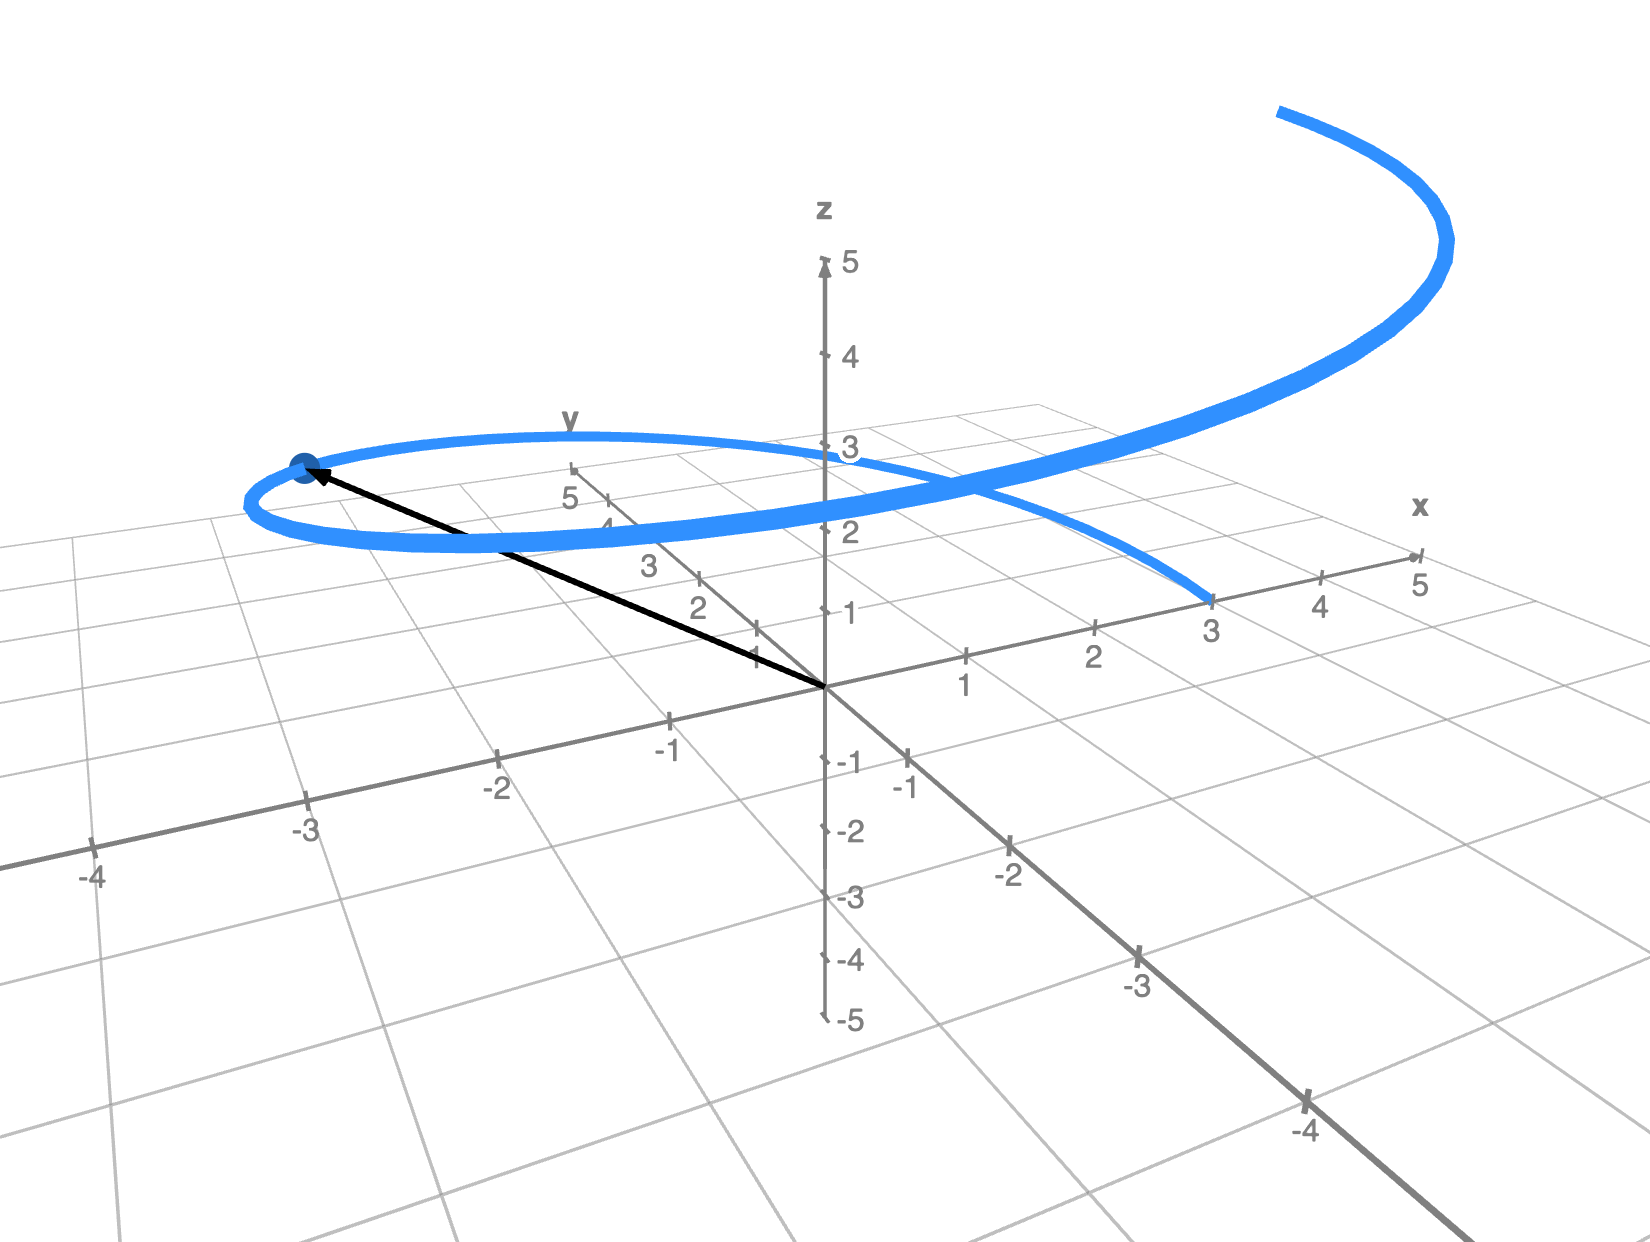
\includegraphics[width=.6\textwidth]{Images/helix.png}
        \caption{Helix.}
    \end{figure}
    \item Here is the plot.
    \begin{figure}[H]
        \centering
        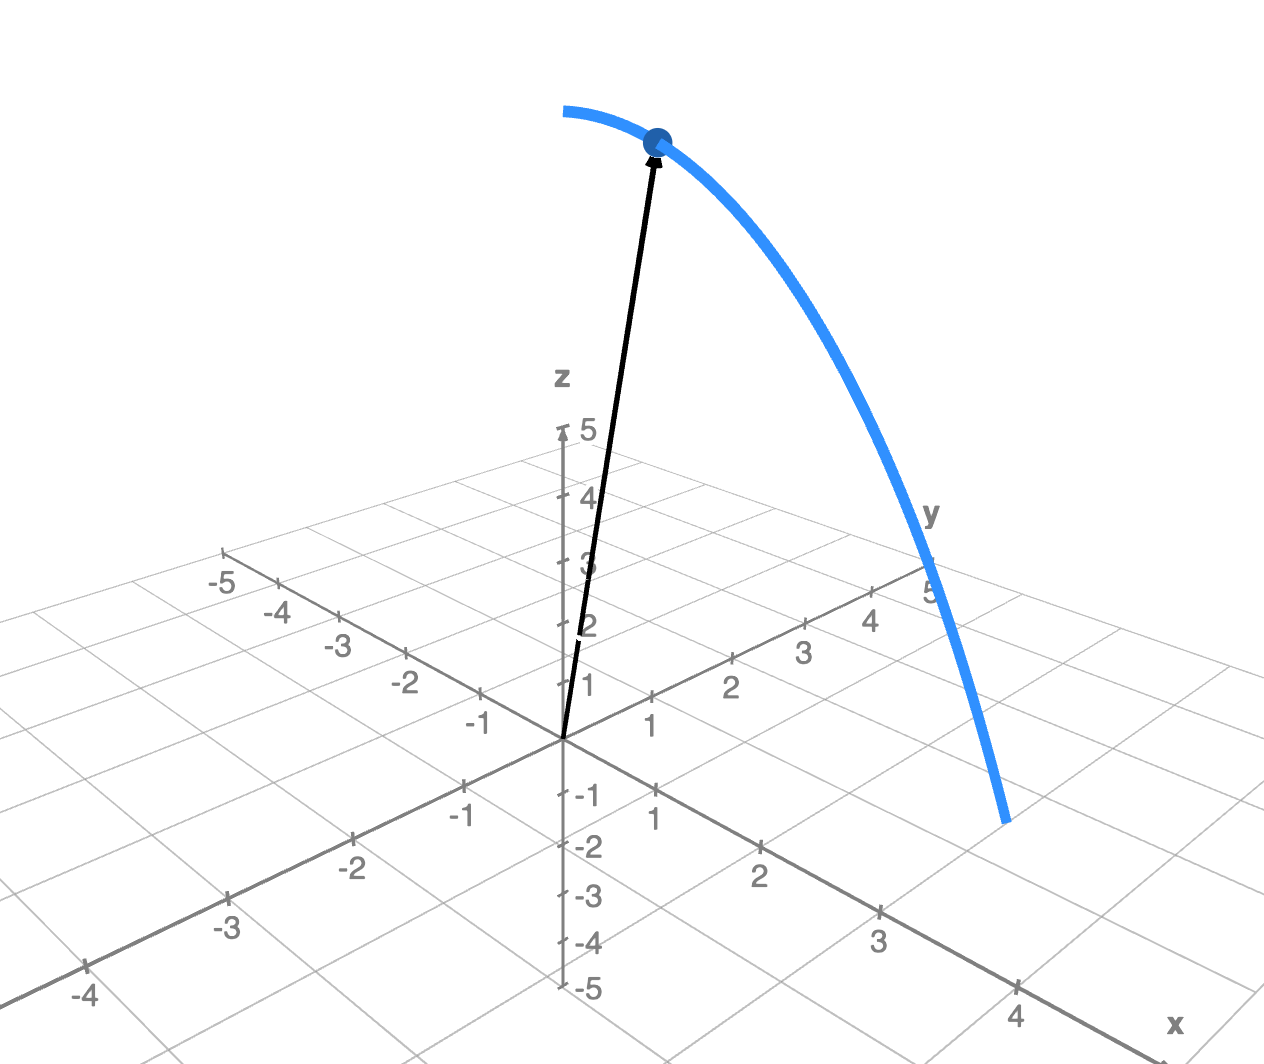
\includegraphics[width=.6\textwidth]{Images/falling_ball.png}
        \caption{Falling ball.}
    \end{figure}
    \item Here is the plot.
    \begin{figure}[H]
        \centering
        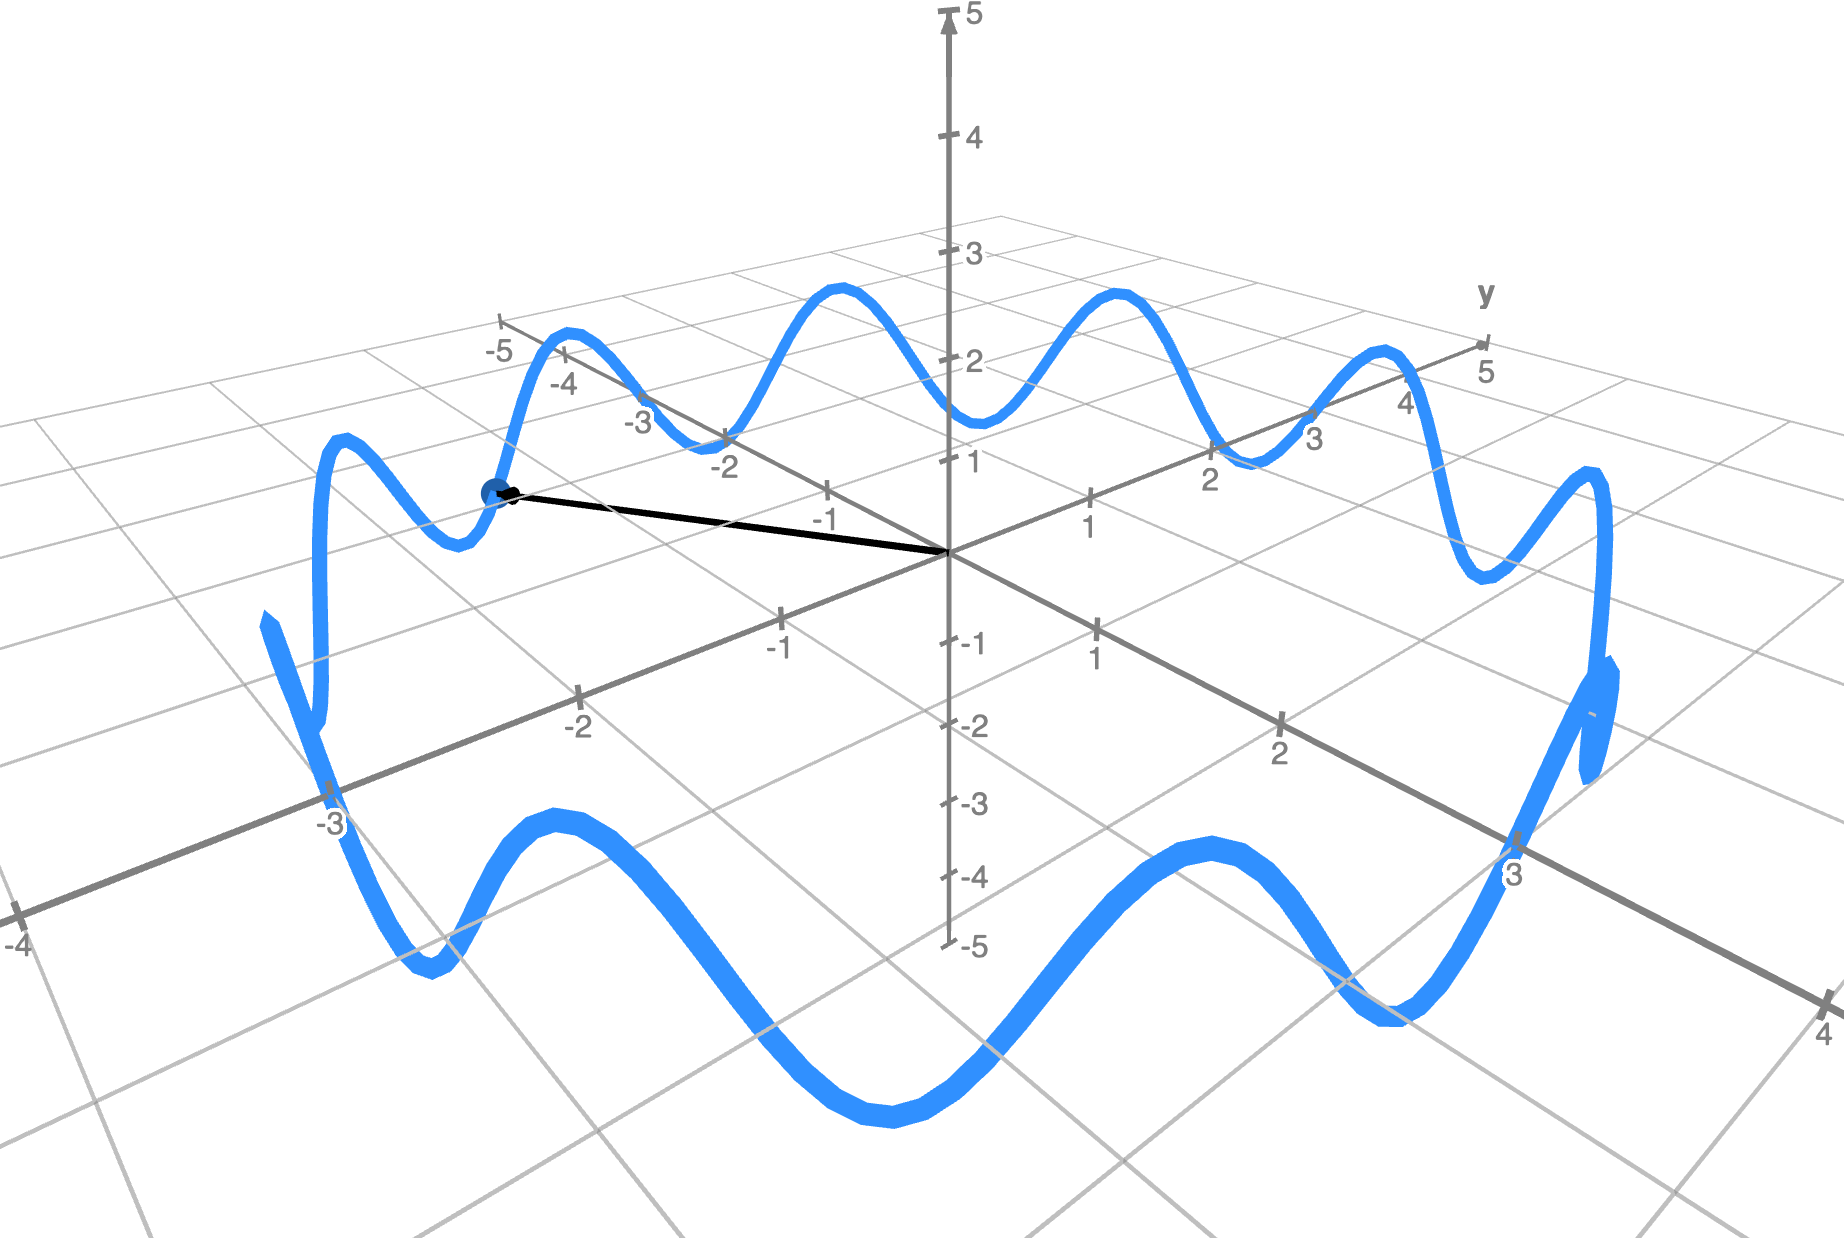
\includegraphics[width=.6\textwidth]{Images/perturbed_orbiter.png}
        \caption{Perturbed orbiter.}
    \end{figure}
\end{enumerate}
And an extra plot of my own. Here, I used the equation
\[
\curvegamma = \begin{pmatrix} (5+3\cos(8t))\cos(t) \\ (5+3\cos(8t))\sin(t) \\ 3\sin(8t) \end{pmatrix}
\]
\begin{figure}[H]
    \centering
    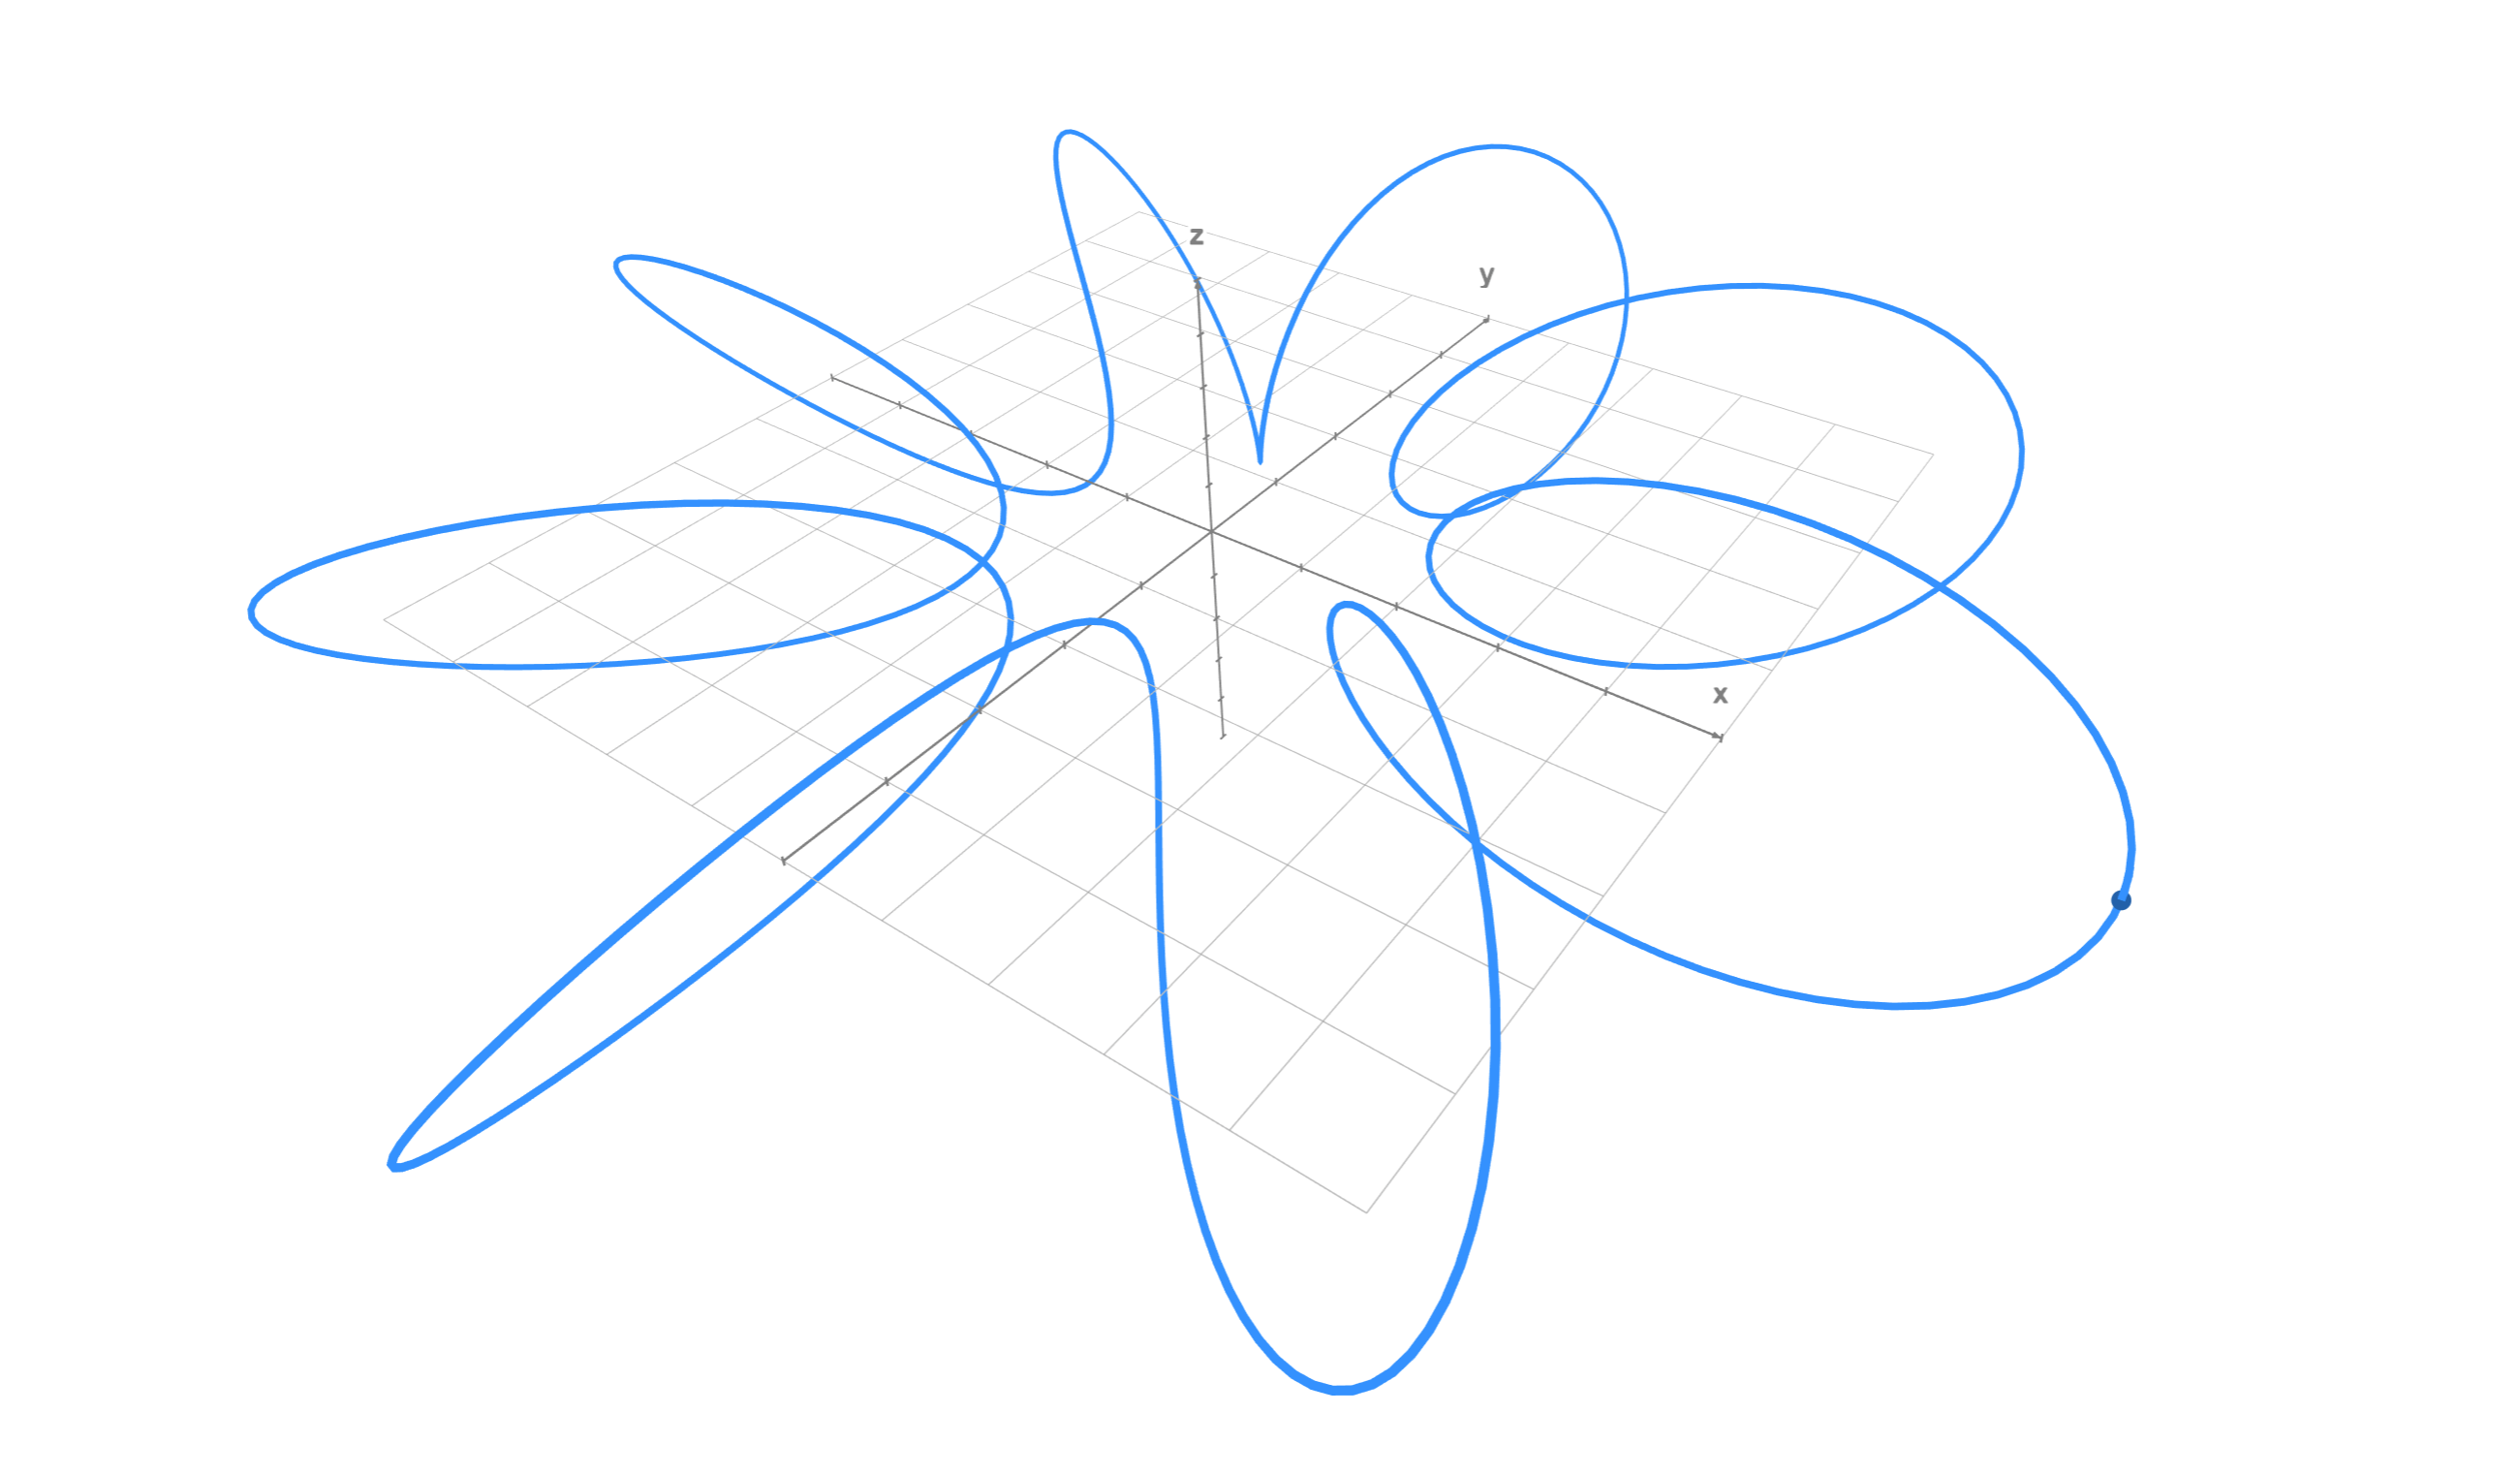
\includegraphics[width=.6\textwidth]{Images/torus_knot.png}
    \caption{A knot that can be tied around a torus (i.e., the surface of a donut).}
\end{figure}
\end{solution}


\newpage
\begin{problem}
The length of a curve is an important notion. In fact, the length of a curve is often related to the energy of some configuration. We can compute the length of a curve over the time $t=t_0$ to $t=t_1$ by integrating the \emph{speed} of the curve over that time.  That is,
\[
l(\curvegamma) = \int_{t_0}^{t_1} \left\|\tangentgamma(t)\right\| dt.
\]
We can compute the \emph{energy} of a curve by taking
\[
E(\curvegamma) = \int_{t_0}^{t_1} \frac{1}{2} \left\| \tangentgamma(t)\right\|^2dt.
\]
\begin{enumerate}[(a)]
	\item Find the length of the Helix from Problem 1 (a).
	\item Find the energy of the Perturbed Orbiter in Problem 1 (c).  Roughly, this corresponds to the potential energy a rubber band stretched this way would have.
\end{enumerate}
\end{problem}
\begin{solution}~
\begin{enumerate}[(a)]
    \item We let $\curvegamma(t) = \begin{pmatrix} 3\cos (t) \\ 3\sin(t) \\ t\end{pmatrix}$ and we go from $t=0$ to $t=2\pi$. Then we have
\[
\tangentgamma(t) =\begin{pmatrix} -3\sin(t) \\ 3\cos(t) \\ 1\end{pmatrix}.
\]
and so
\[
\left\|\tangentgamma(t)\right\| = \sqrt{(-3\sin (t))^2+(3\cos (t))^2+1^2} = \sqrt{10},
\]
since $\sin^2(t)+\cos^2(t)=1$.

Now we integrate to find
\begin{align*}
    l(\curvegamma) &= \int_0^{2\pi} \sqrt{10}dt\\
    &= \sqrt{10} t|_0^{2\pi}\\
    &= 2\pi \sqrt{10}.
\end{align*}
    \item Here we have $\curvegamma(t)=\begin{pmatrix} 3\cos(t) \\ 3\sin(t) \\ \sin(10t)\end{pmatrix}$ starting from $t=0$ to $t=2\pi$. Then we have
    \[
    \tangentgamma(t)=\begin{pmatrix} -3\sin(t) \\ 3\cos(t) \\ 10\cos(10t)\end{pmatrix}
    \]
    and so
    \[
    \left\|\tangentgamma'(t)\right\| = \sqrt{(-3\sin(t))^2+(3\cos(t))^2+(10\cos(10t))^2} = \sqrt{9+100\cos^2(10t)}.
    \]
    This is not a function that can be integrated without some trigonometric substitutions.  If you're interested, you can look at integration using trigonometric substitutions, but I will not go into it. Instead, I'd argue it's good practice for us to get more used to using technology to help solve our problems.  So, we wish to evaluate the integral
    \[
    E(\gamma) = \int_0^{2\pi} \frac{1}{2}(9+100\cos^2(10t))dt.
    \]
	Then we can type into WolframAlpha
	\begin{verbatim}
	integrate[(1/2)(9+100cos^2(10t)),{t,0,2*pi}]
	\end{verbatim}
    
    Using this, we find
    \[
    E(\gamma)=59\pi.
    \]

\end{enumerate}
\end{solution}

\newpage
\begin{problem}
Given a scalar field of two variables $F(x,y)$, we can create an object called the \emph{graph} of $F(x,y)$ by plotting the set of points $(x,y,F(x,y))$. In fact, you have done this many times in your life. For example, you have consistently plotted the graph of a function $f(x)$ by plotting $(x,f(x))$ in the plane!  

Using GeoGebra, plot the graph of the following functions. Print these off and include them.  Also, describe the what the graph of the function does as we move along the $x$-axis, the $y$-axis, and along the line $y=x$. For each, use the range $-3\leq x \leq 3$ and $-3\leq y \leq 3$.
\begin{enumerate}[(a)]
	\item $F(x,y) = \frac{4xy}{1+x^2+y^2}$.
	\item $G(x,y) = \sin(xy)$.
	\item $H(x,y) = \frac{-x^2-y^2}{5}$.
\end{enumerate}
\end{problem}
\begin{solution}~
\begin{enumerate}[(a)]
    \item Below is the graph of the function $F(x,y)$.
    \begin{figure}[H]
        \centering
        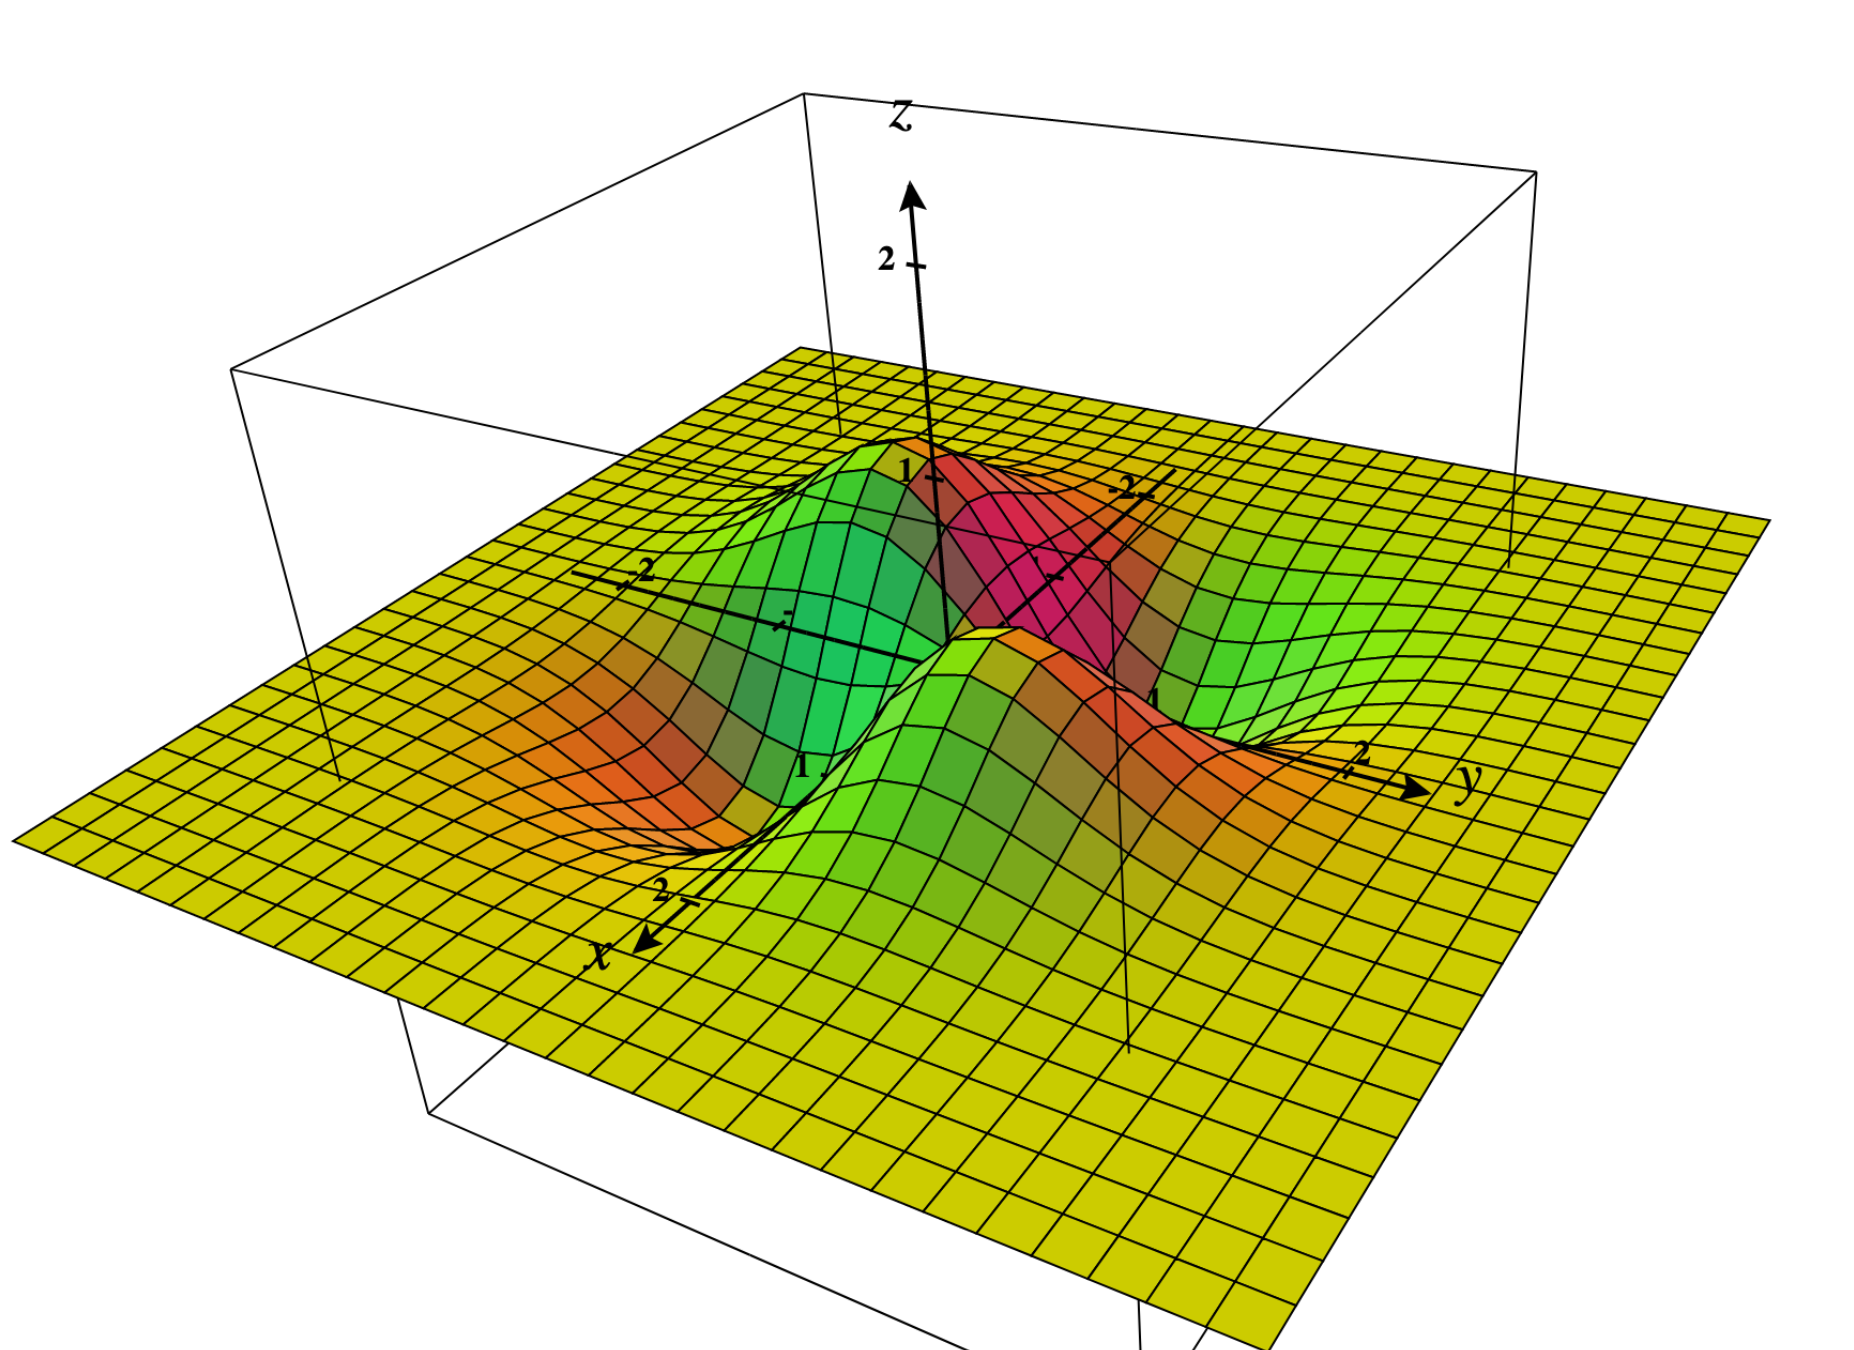
\includegraphics[width=.6\textwidth]{Images/4a.png}
        \caption{The graph of $F(x,y)$.}
    \end{figure}
    If we move along the $x$-axis, then we have that $y=0$ and thus our function takes the form
    \[
    F(x,0) = \frac{4x\cdot 0}{1+x^2+0^2} = 0.
    \]
    Thus, along this axis the function is a constant zero. Similarly, if we take $x=0$ we have that $F(0,y)=0$ and our function is again constantly zero along this axis. Instead, if we take the function along the $y=x$ line, then we have
    \[
    F(x,x) = \frac{4x^2}{1+2x^2}
    \]
    We can plot this function as a single variable graph in the $(x=y)z$-plane by:
    \begin{figure}[H]
    	\centering
    	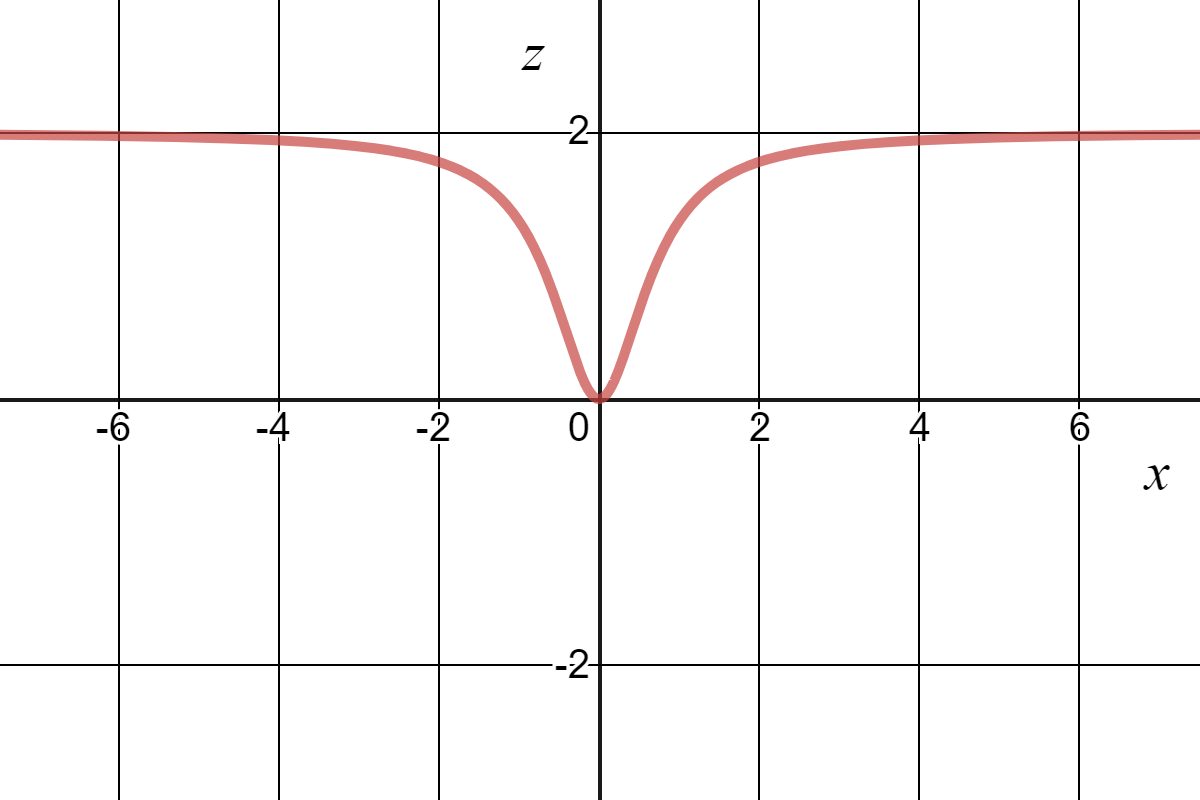
\includegraphics[width=.6\textwidth]{Images/3a_y=x.png}
    	\caption{The graph of $F(x,x)$ in the $xz$-plane.}
    \end{figure}
    \item Below is the graph of the function $G(x,y)$.
    \begin{figure}[H]
        \centering
        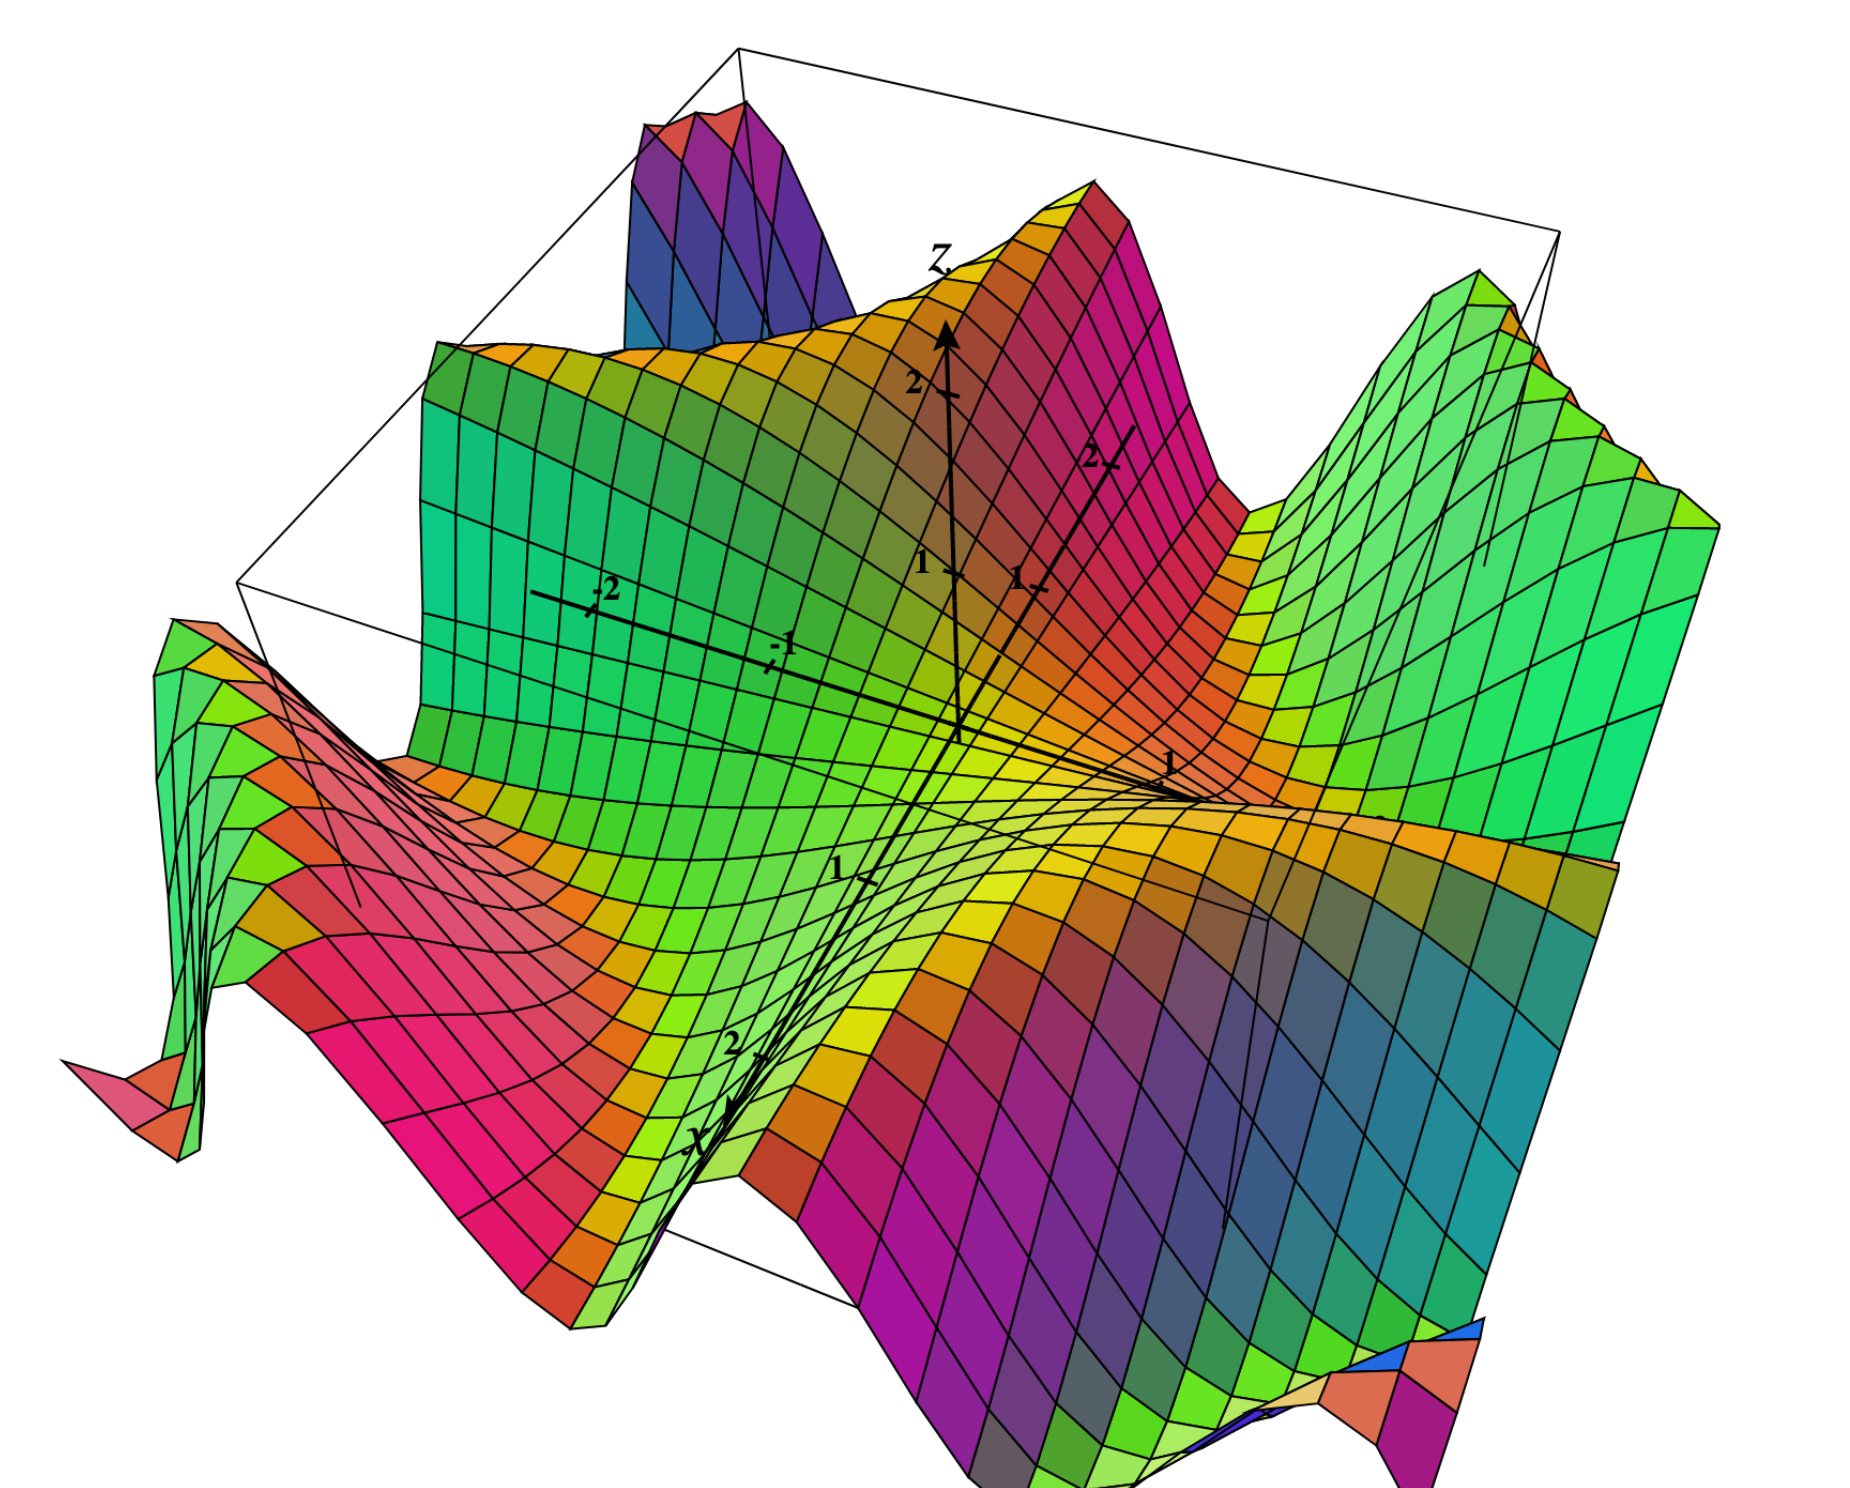
\includegraphics[width=.6\textwidth]{Images/4b.png}
        \caption{The graph of $G(x,y)$.}
    \end{figure}
    If we move along the $x$-axis, we take $y=0$ and thus
    \[
    G(x,0) = \sin(0) = 0.
    \]
    Hence, our function is constantly zero on this axis.  Similarly, if we take the function on the $y$-axis, then $x=0$ means
    \[
    G(0,y) = 0.
    \]
    Lastly, if we take $y=x$, then
    \[
    G(x,x) = \sin(x^2),
    \]
    which we can graph in the $(x=y)z$-plane by:
        \begin{figure}[H]
        	\centering
        	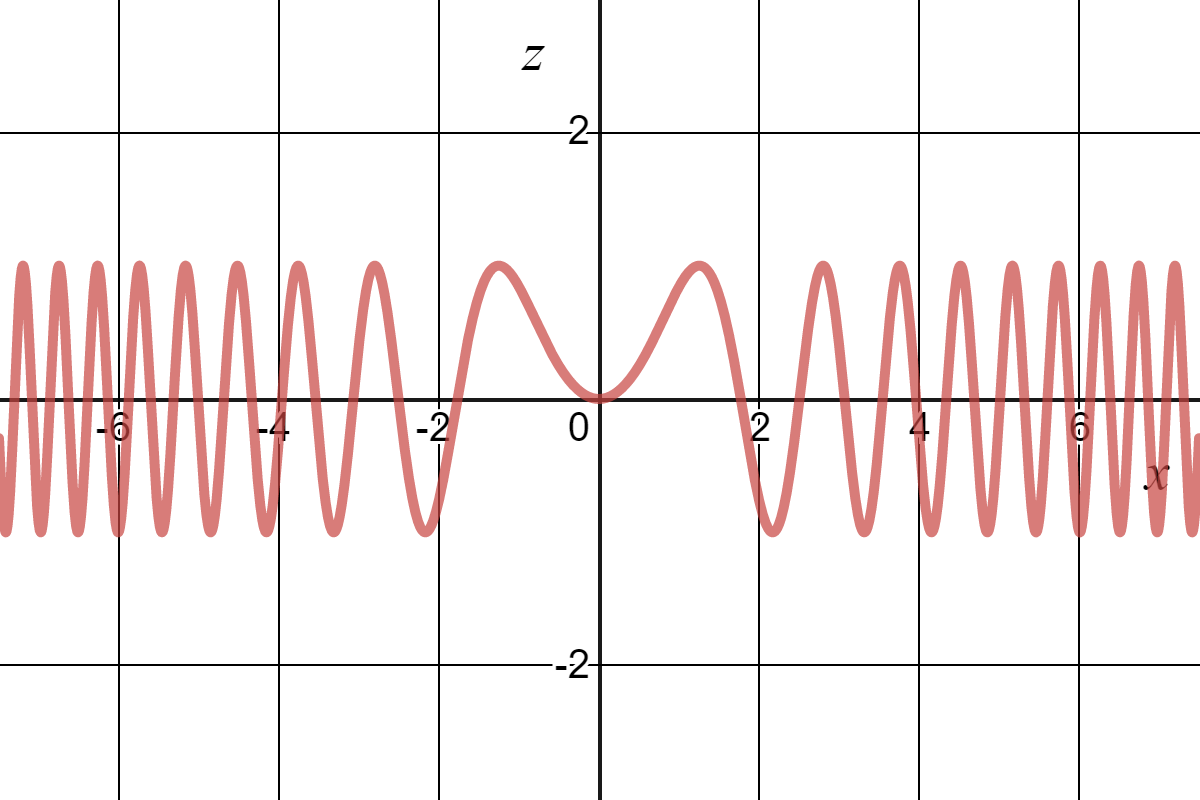
\includegraphics[width=.6\textwidth]{Images/3b_y=x.png}
        	\caption{The graph of $G(x,x)$ in the $xz$-plane.}
        \end{figure}
    \item Below is the graph of $H(x,y)$.
    \begin{figure}[H]
        \centering
        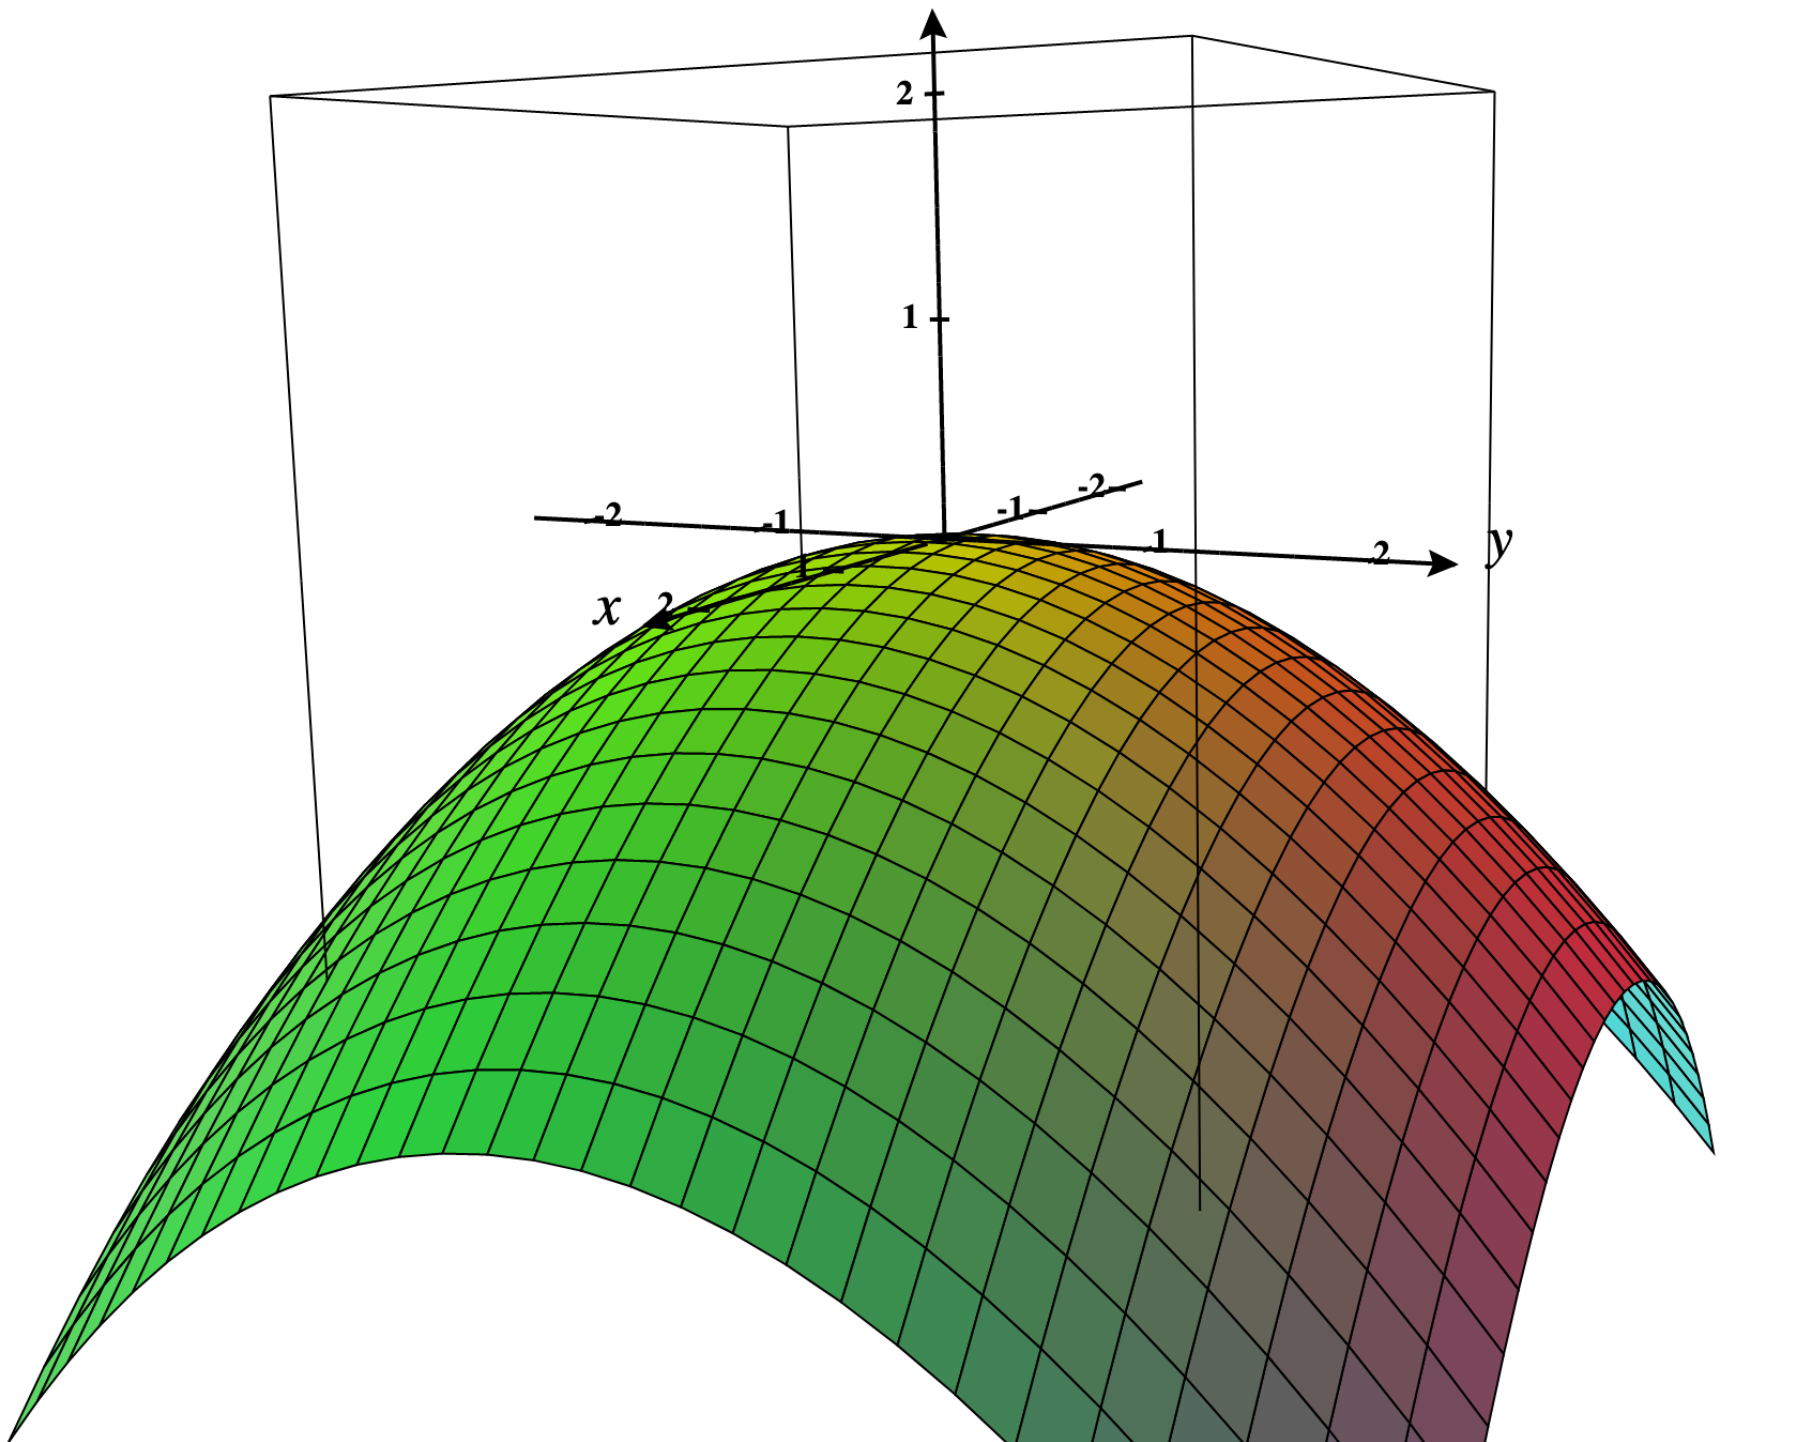
\includegraphics[width=.6\textwidth]{Images/4c.png}
        \caption{The graph of $H(x,y)$.}
    \end{figure}
    Here if we consider the function along the $x$-axis, we have
    \[
    H(x,0)= \frac{-x^2}{5},
    \]
    which is a parabola in the $xz$-plane. Similarly, on the $y$-axis, we have
    \[
    H(0,y) = \frac{-y^2}{5},
    \]
    which is the same parabola but in the $yz$-plane. Lastly, letting $x=y$ we get
    \[
    H(x,x) = \frac{-2x^2}{5},
    \]
    which is a steeper parabola in the $(x=y)z$-plane.
\end{enumerate}
\end{solution}

\newpage
\begin{problem}
For this problem, let us consider a family of scalar fields of varying dimensionality.  We will seek out an understanding of the level sets and how to relate these to the derivatives of a scalar field. For each part, compute the set of points such that $f(\vecx)=\frac{1}{2}$, $f(\vecx)=1$, $f(\vecx)=2$, and $f(\vecx)=3$ and plot these sets. 

Compute as well the vector of partial derivatives (referred to as the \emph{gradient vector}) which we write as
\[
\nablavec f(\vecx) = \begin{pmatrix} \frac{\partial f}{\partial x_1} \\ \frac{\partial f}{\partial x_2} \\ \vdots \\ \frac{\partial f}{\partial x_n}\end{pmatrix}.
\]
in $\R^n$. Draw the gradient vector on your plots at a three different points for each part.
\begin{enumerate}[(a)]
	\item Consider the 1-dimensional scalar field 
	\[
	f(x) = \frac{1}{|x|}=\frac{1}{\sqrt{x^2}}.
	\]
	Here each level set will be made up of distinct points.
	\item Consider the 2-dimensional scalar field
	\[
	f(x) = \frac{1}{|\vec{x}|} = \frac{1}{\sqrt{x^2+y^2}}.
	\]
	Here each level set will be a curve.
	\item Consider the 3-dimensional scalar field
		\[
		f(x) = \frac{1}{|\vec{x}|} = \frac{1}{\sqrt{x^2+y^2+z^2}}.
		\]
		Here each level set will be a surface.
\end{enumerate}
\end{problem}
\begin{solution}~
\begin{enumerate}[(a)]
    \item We first solve this problem algebraically then we'll deal with the plots.  We have
    \begin{align*}
        f(x)&=c\\
        \iff \frac{1}{\sqrt{x}^2} &= c\\
        \iff \sqrt{x^2}&=\frac{1}{c}\\
        \iff x^2&= \frac{1}{c^2}\\
        \iff x &= \pm \frac{1}{c}.
    \end{align*}
    Now using this, we find that the level points follow:
    \begin{align*}
        \textrm{For $c_0=\frac{1}{2}$:~}\quad x&=\pm 2\\
        \textrm{For $c_1=1$:~}\quad x&=\pm 1\\
        \textrm{For $c_2=2$:~}\quad x&=\pm \frac{1}{2}\\
        \textrm{For $c_3=3$:~}\quad x&=\pm \frac{1}{3}.\\
    \end{align*}
    Here are the plots.
    \begin{figure}[H]
        \centering
        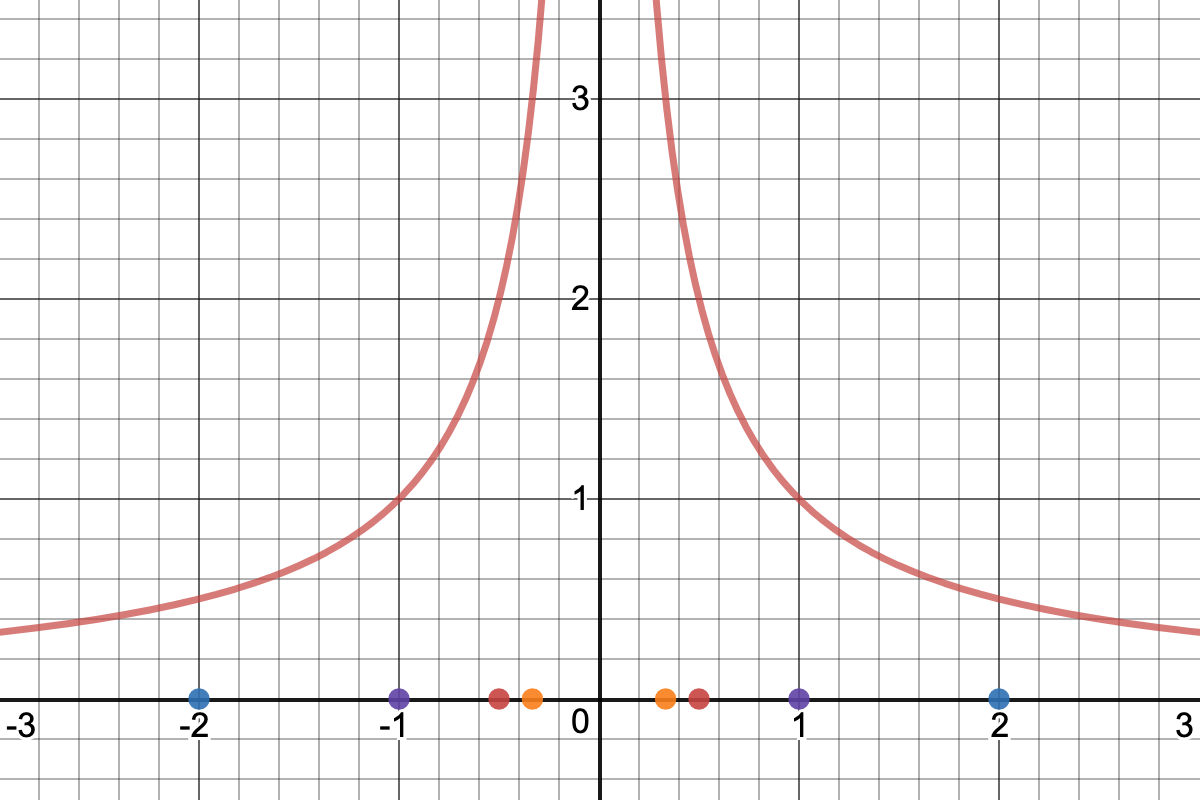
\includegraphics[width=.6\textwidth]{Images/level_points.png}
        \caption{Graph of $f(x)$ with level points on the $x$-axis.}
    \end{figure}
    \item Let's repeat the same process as in (a). We take
    \begin{align*}
        f(x,y)&=c\\
        \iff \frac{1}{\sqrt{x^2+y^2}}&= c\\
        \iff \sqrt{x^2+y^2}&=\frac{1}{c}\\
        \iff x^2+y^2 &= \frac{1}{c^2},
    \end{align*}
    which is the equation for a circle of radius $\frac{1}{c}$. Now using this, we find that the level curves follow:
    \begin{align*}
        \textrm{For $c_0=\frac{1}{2}$:~}\quad x^2+y^2&=2\\
        \textrm{For $c_1=1$:~}\quad x^2+y^2&=1\\
        \textrm{For $c_2=2$:~}\quad x^2+y^2&=\frac{1}{4}\\
        \textrm{For $c_3=3$:~}\quad x^2+y^2&=\frac{1}{9}.\\
    \end{align*}
    Here are the plots.
    \begin{figure}[H]
        \centering
        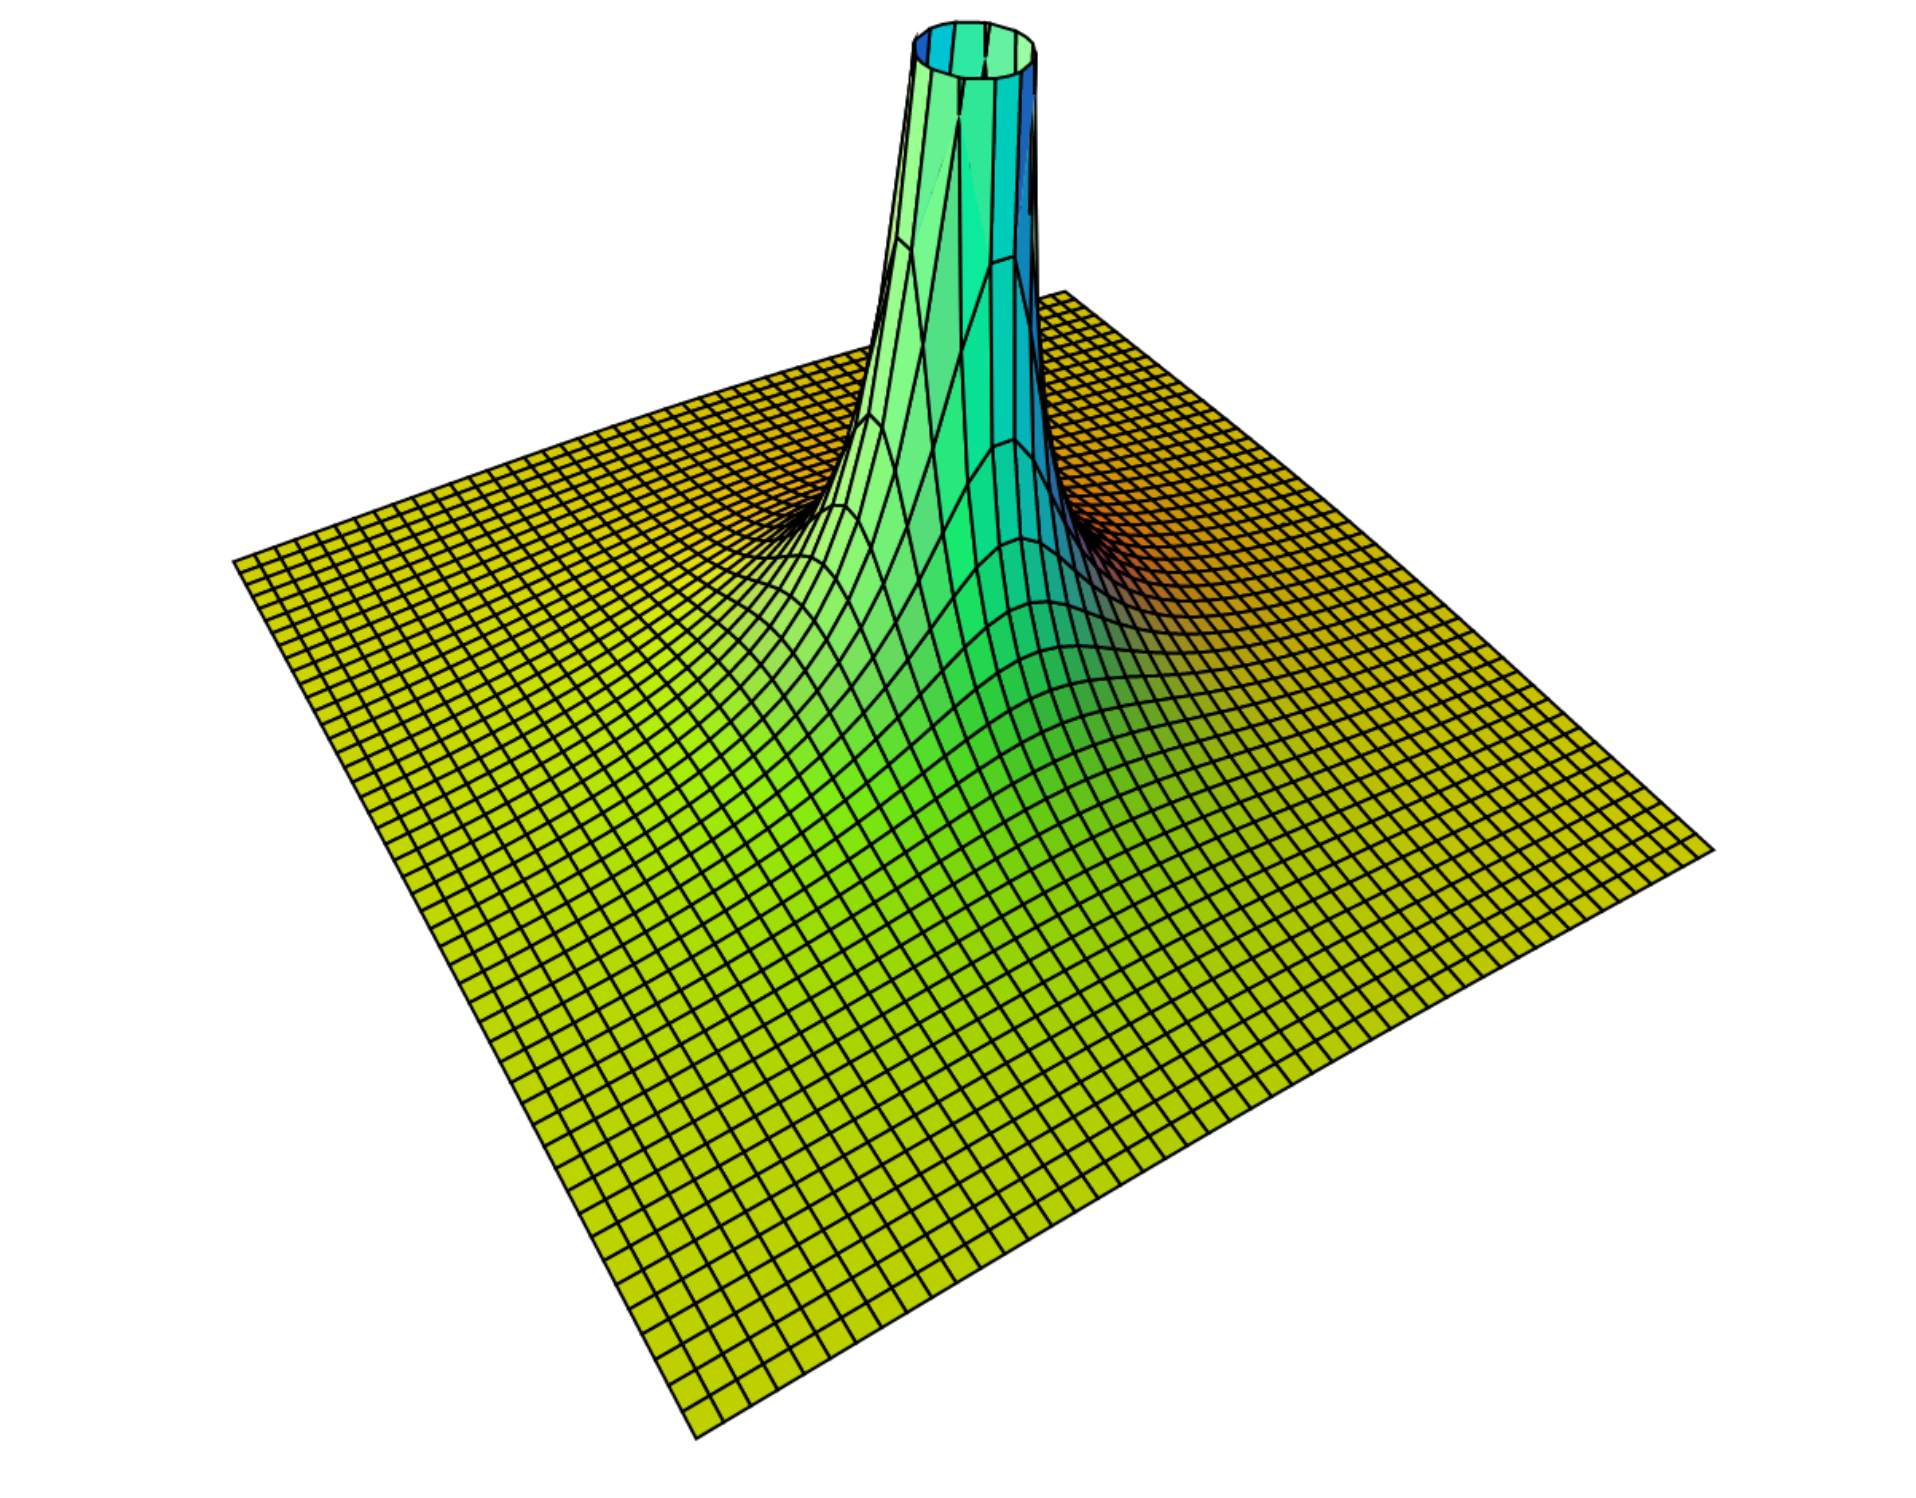
\includegraphics[width=.6\textwidth]{Images/level_curve_surface.png}
        \caption{The graph of the function $f(x,y)$.}
    \end{figure}
    \begin{figure}[H]
        \centering
        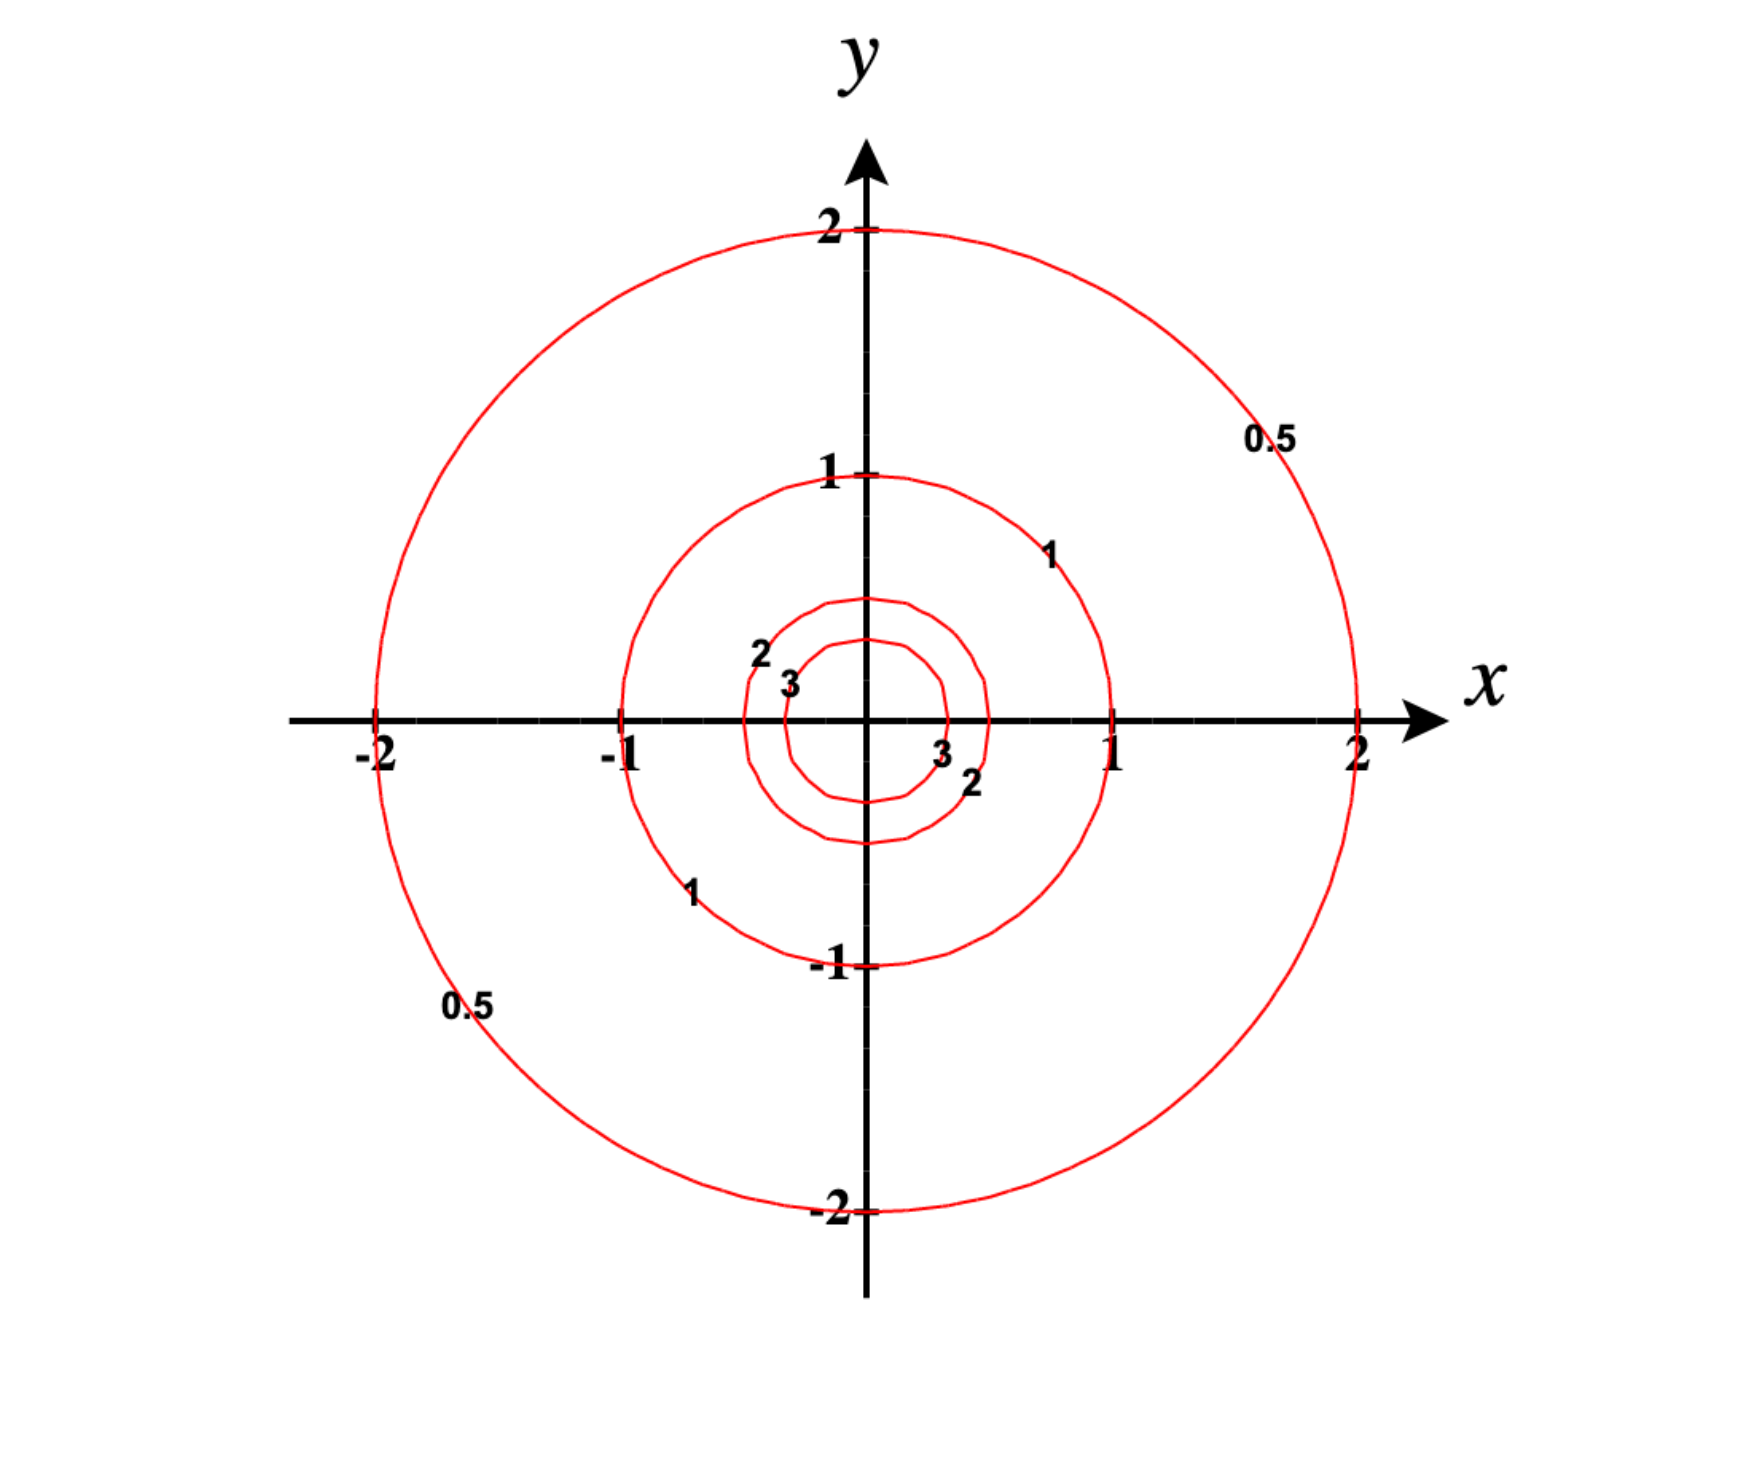
\includegraphics[width=.6\textwidth]{Images/level_curves.png}
        \caption{The level curves for the function $f(x,y)$.}
    \end{figure}
    \item Let's repeat the process one last time, so we have
    \begin{align*}
            f(x,y,z)&=c\\
        \iff \frac{1}{\sqrt{x^2+y^2+z^2}}&= c\\
        \iff \sqrt{x^2+y^2+z^2}&=\frac{1}{c}\\
        \iff x^2+y^2+z^2 &= \frac{1}{c^2},
    \end{align*}
    which is the equation for a sphere of radius $\frac{1}{c}$.  Then the level surfaces follow:
        \begin{align*}
        \textrm{For $c_0=\frac{1}{2}$:~}\quad x^2+y^2+z^2&=2\\
        \textrm{For $c_1=1$:~}\quad x^2+y^2+z^2&=1\\
        \textrm{For $c_2=2$:~}\quad x^2+y^2+z^2&=\frac{1}{4}\\
        \textrm{For $c_3=3$:~}\quad x^2+y^2+z^2&=\frac{1}{9}.\\
    \end{align*}
    Here are the plots
    \begin{figure}[H]
        \centering
        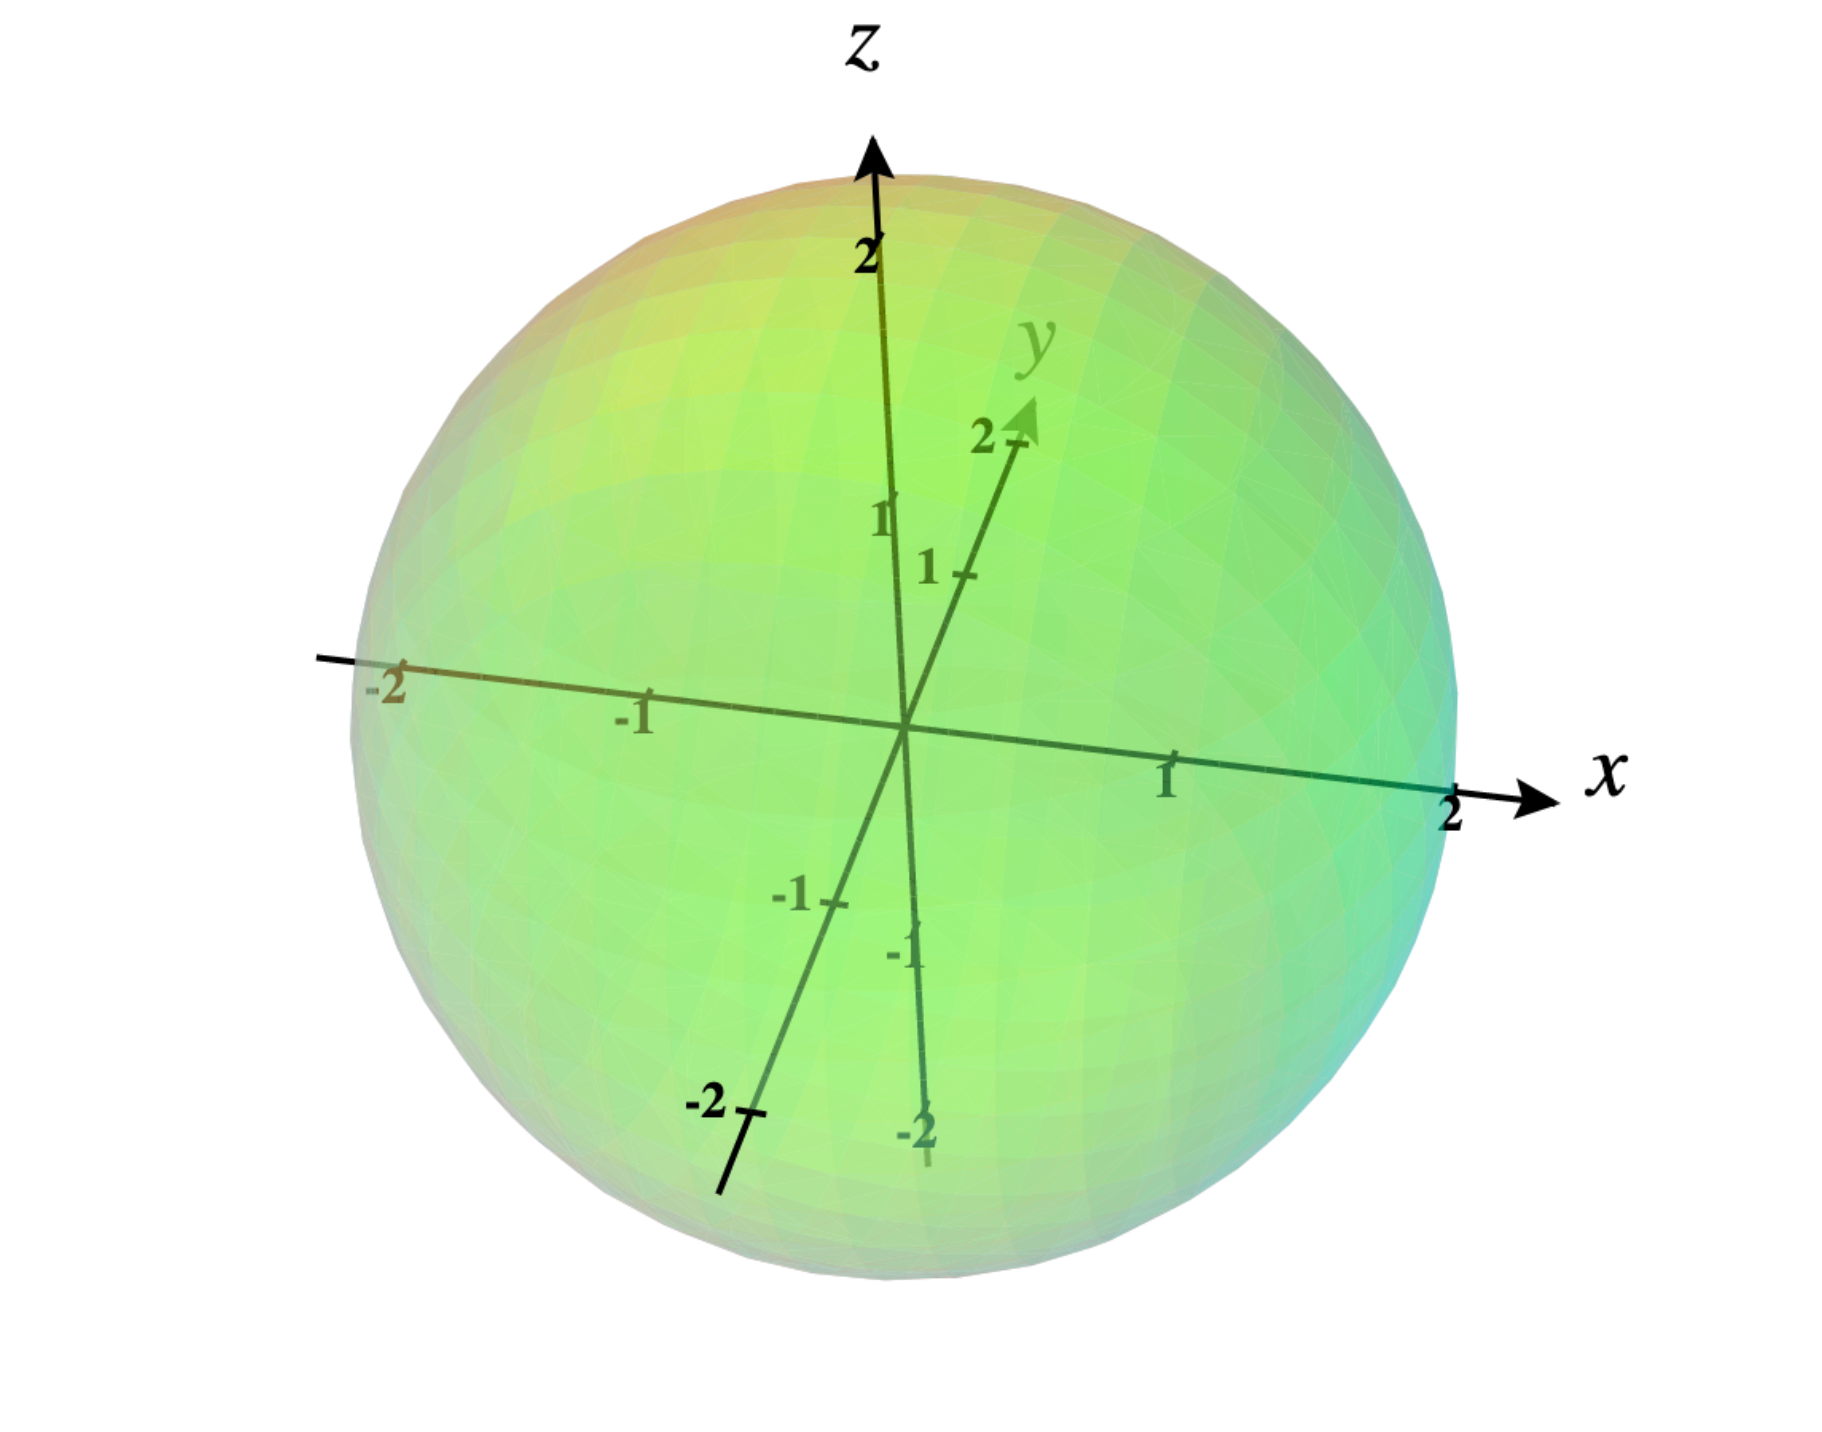
\includegraphics[width=.6\textwidth]{Images/level_surface_c0.png}
        \caption{Level surface for $f(x,y,z)=c_0$.}
    \end{figure}
        \begin{figure}[H]
        \centering
        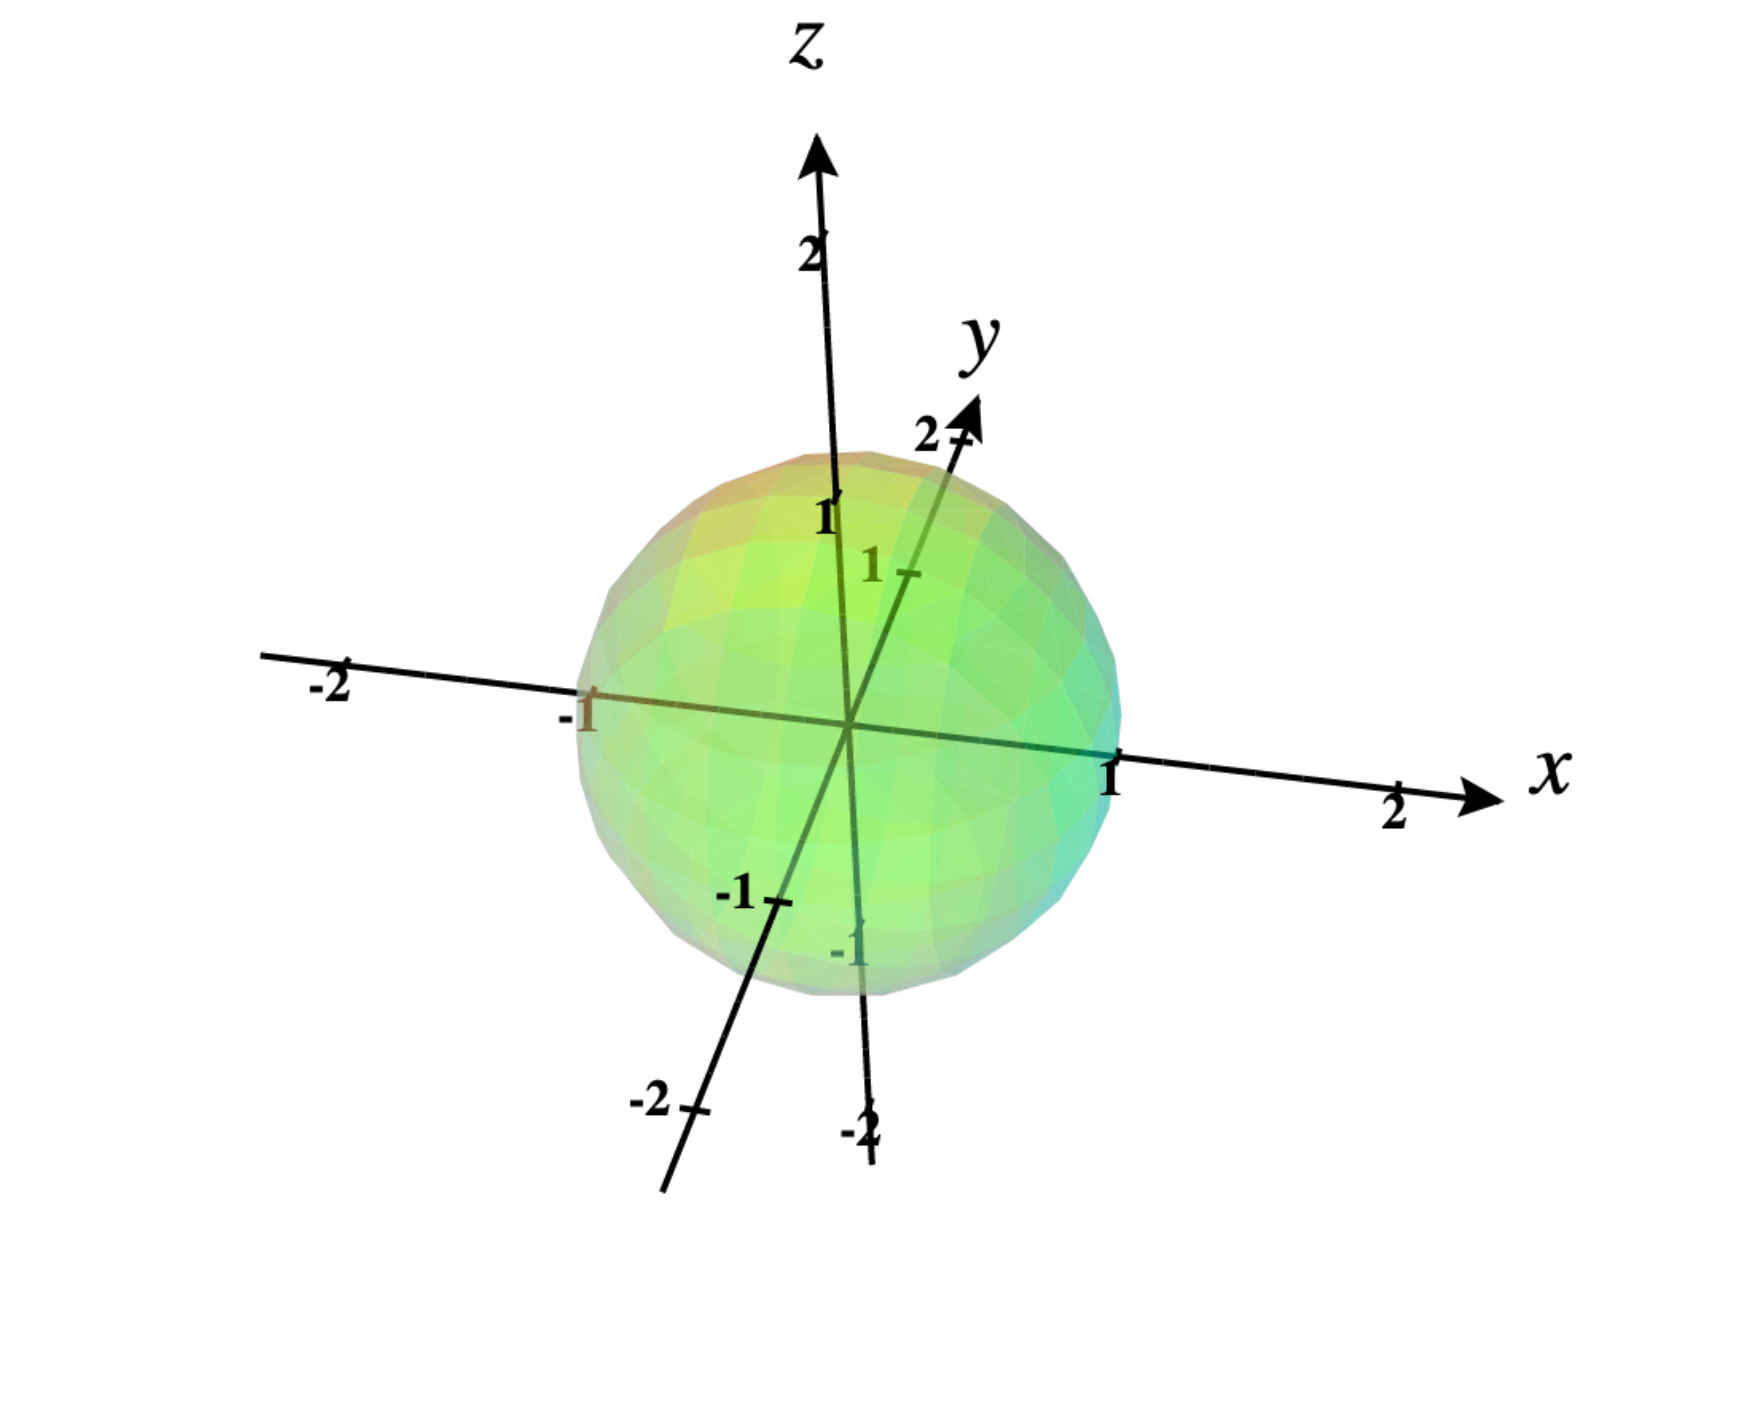
\includegraphics[width=.6\textwidth]{Images/level_surface_c1.png}
        \caption{Level surface for $f(x,y,z)=c_1$.}
    \end{figure}
        \begin{figure}[H]
        \centering
        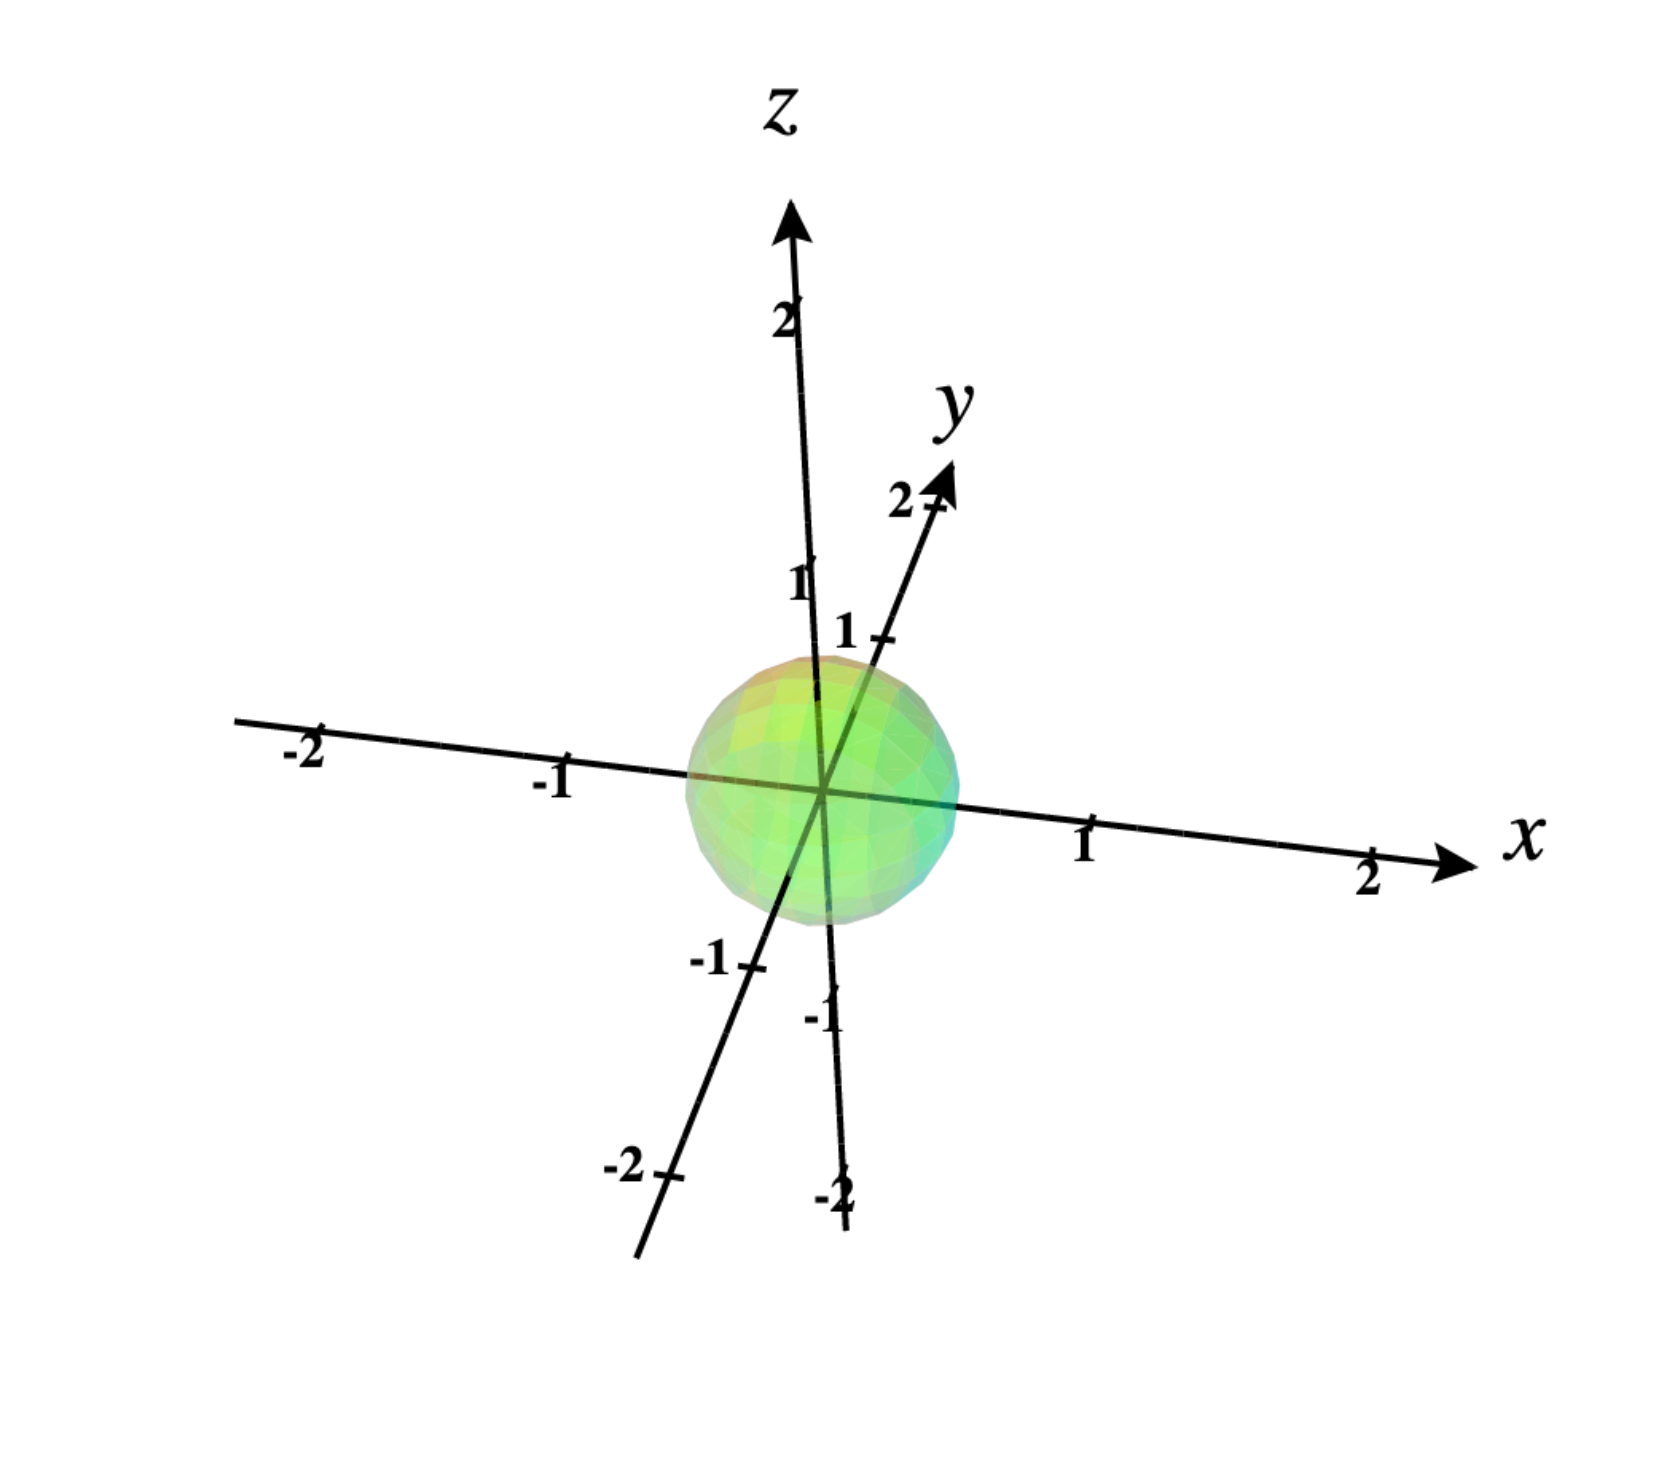
\includegraphics[width=.6\textwidth]{Images/level_surface_c2.png}
        \caption{Level surface for $f(x,y,z)=c_2$.}
    \end{figure}
        \begin{figure}[H]
        \centering
        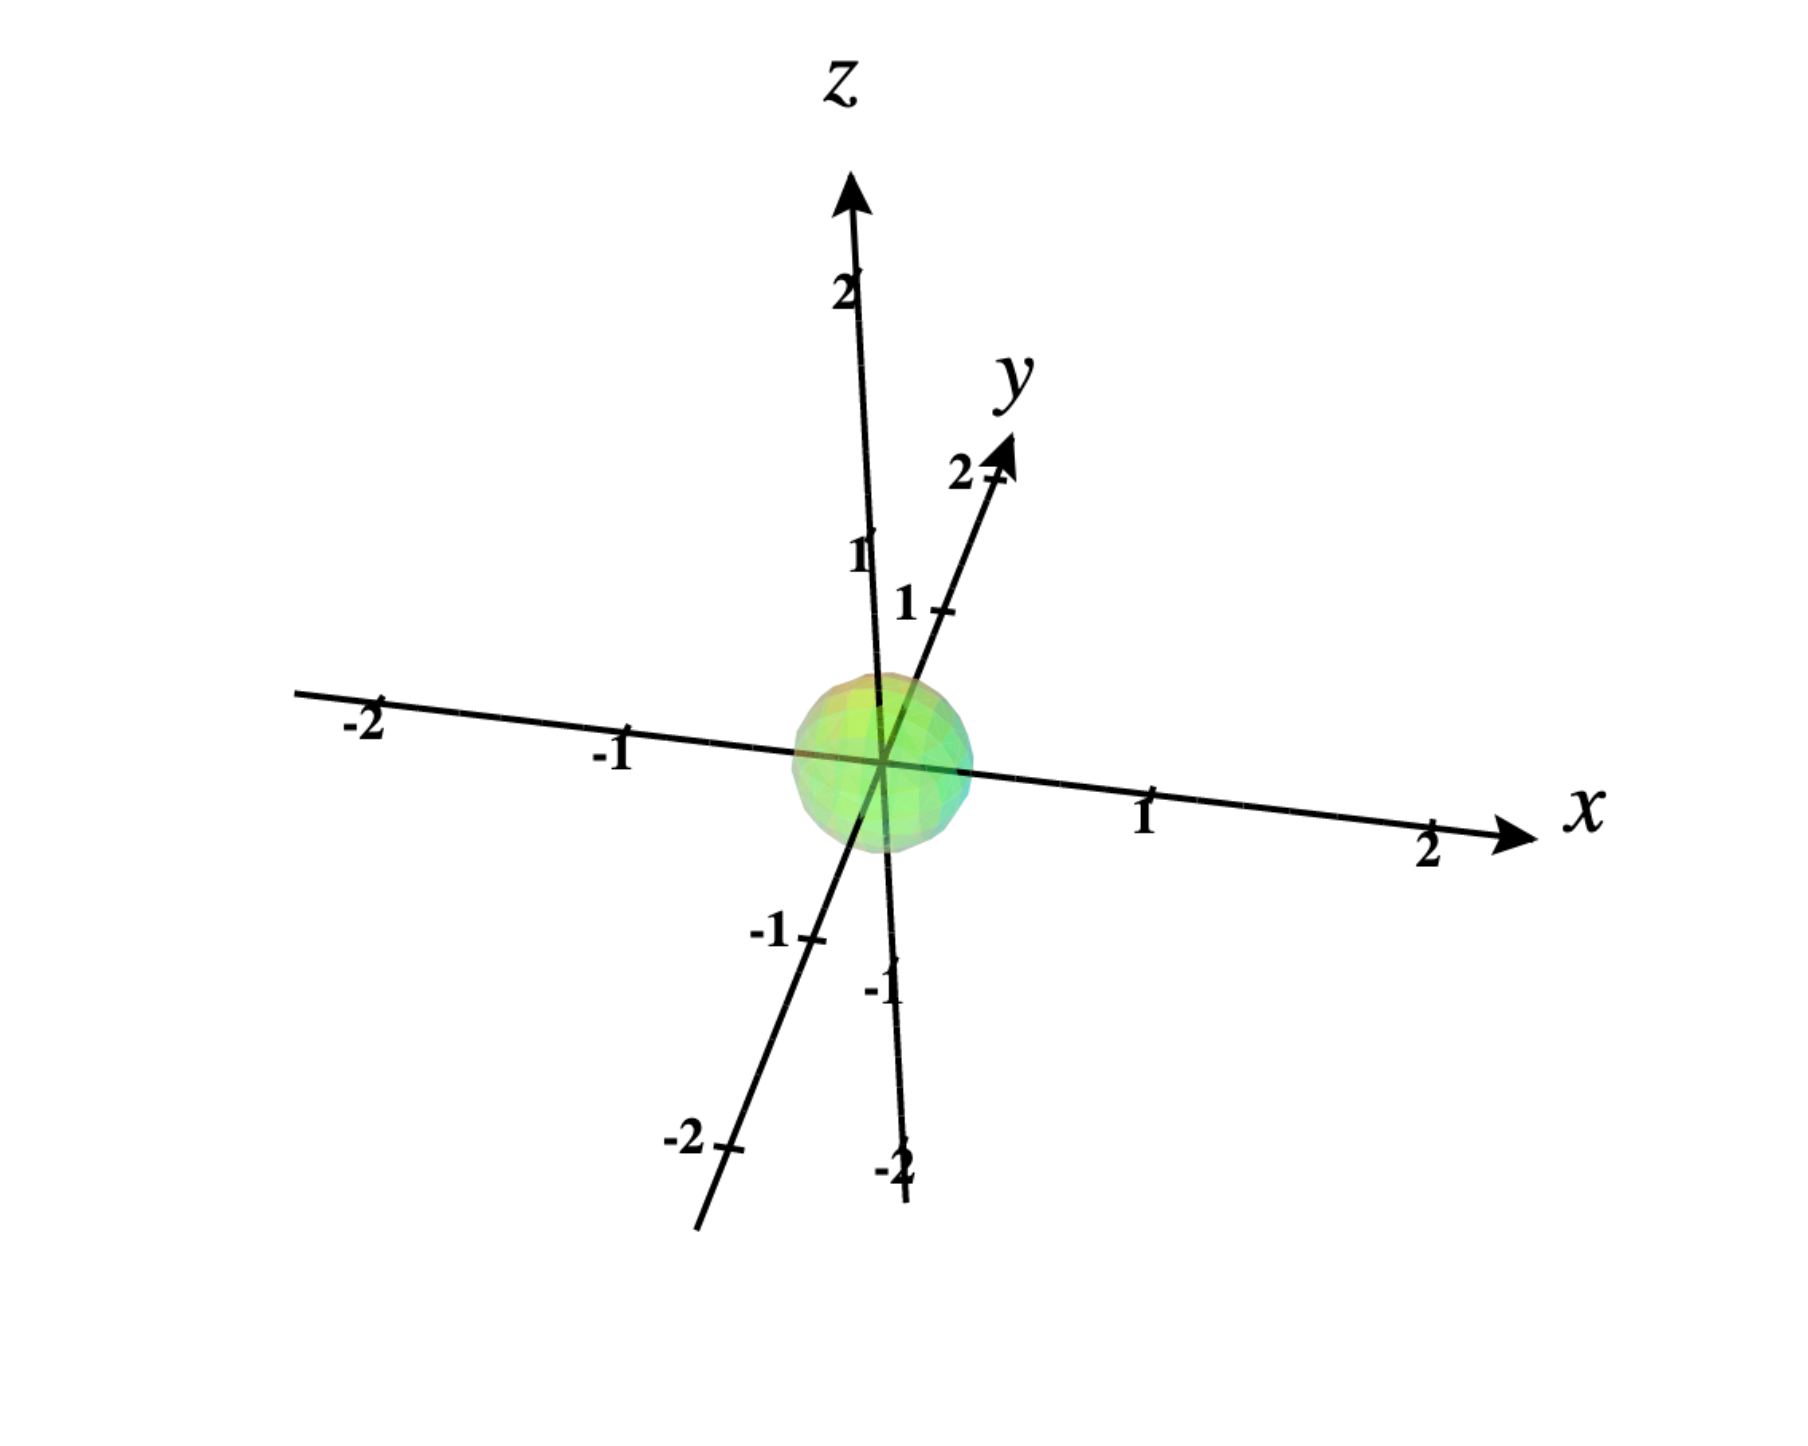
\includegraphics[width=.6\textwidth]{Images/level_surface_c3.png}
        \caption{Level surface for $f(x,y,z)=c_3$.}
    \end{figure}
\end{enumerate}
One can think of these level sets as the sets of constant energy. For example, if this function $f(x,y,z)$ describes the potential energy (which this function does for the gravitational and electrostatic force), then the level sets correspond to the circular orbits of particles in this potential field. 
\end{solution}

\newpage
\begin{problem}
Consider the two dimensional scalar field $T(x,y)=x+y$ that describes the temperature on the square plate $\Omega$ given by the set $0\leq x,y \leq 1$.  Compare the two answers you get!
\begin{enumerate}[(a)]
	\item Compute the integral
	\[
	\int_\Omega T(x,y)d\Omega.
	\]
	\item Let $\curvegamma$ be the curve that traverses the boundary of the square plate in the counterclockwise direction.  Compute
	\[
	\int_{\curvegamma} T(\curvegamma)d\curvegamma. 
	\]
\end{enumerate}
\end{problem}
\begin{solution} ~
	\begin{enumerate}[(a)]
		\item We take
		\begin{align*}
			\iint_\Omega T(x,y)d\Omega &= \int_0^1 \int_0^1 x+y dxdy\\
			&= \int_0^1 \left.\left(\frac{1}{2}x^2+xy\right)\right\vert_0^1 dy\\
			&= \int_0^1 \frac{1}{2} + y dy\\
			&= \left.\left(\frac{1}{2}y + \frac{1}{2}y^2\right)\right\vert_0^1\\
			&= 1.
		\end{align*}
		\item	First, note that there are four straight curves that parameterize the boundary of the plate.  Namely, we can choose the parameterizations 
		\[
		\curvegamma_1(t) = \begin{pmatrix} t \\ 0 \end{pmatrix} \quad \curvegamma_2(t) = \begin{pmatrix} 1 \\ t \end{pmatrix} \quad \curvegamma_1(t) = \begin{pmatrix} 1-t \\ 1 \end{pmatrix} \quad \curvegamma_1(t) = \begin{pmatrix} 0 \\ 1-t \end{pmatrix},
		\]
		Note that there are many other parameterizations that work. We can see the chosen curves in this figure:
		\begin{figure}[H]
			\centering
			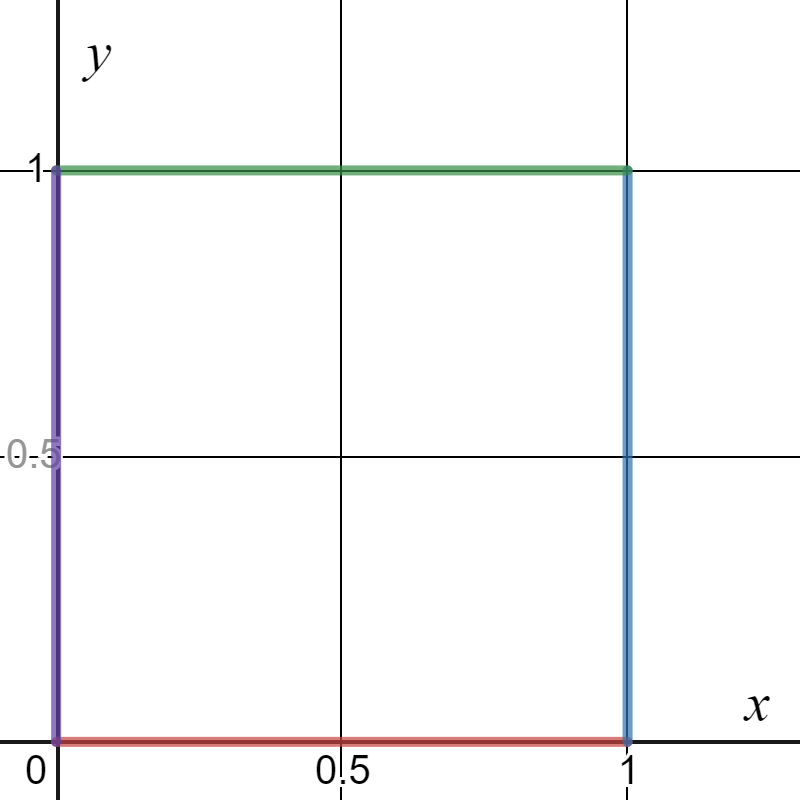
\includegraphics[width=.6\textwidth]{Images/plate_boundary.png}
		\end{figure}
		Thus, our integral can be written as
		\[
		\int_{\curvegamma} T(\curvegamma) d\curvegamma = \int_{\curvegamma_1} T(\curvegamma) d\curvegamma_1 + \int_{\curvegamma_2} T(\curvegamma) d\curvegamma_2 + \int_{\curvegamma_3} T(\curvegamma) d\curvegamma_3 + \int_{\curvegamma_4} T(\curvegamma) d\curvegamma_4.
		\]
		Then, we can compute each integral on the right hand side.
		\begin{align*}
			\int_{\curvegamma_1} T(\curvegamma_1) d\curvegamma_1 &= \int_0^1 T(\curvegamma_1(t))\left|\tangentgamma_1(t)\right|dt\\
			&= \int_0^1 T(t,0) dt\\
			&= \int_0^1 t dt\\
			&= 1.
		\end{align*}
		Similarly, 
		\begin{align*}
				\int_{\curvegamma_2} T(\curvegamma_2) d\curvegamma_2 &= \int_0^1 T(\curvegamma_2(t))\left|\tangentgamma_2(t)\right|dt\\
				&= \int_0^1 T(1,t) dt\\
				&= \int_0^1 1+t dt\\
				&= \left.\left(t+\frac{1}{2}t^2\right)\right\vert_0^1\\
				&= \frac{3}{2}.
		\end{align*}	
		Again,
		\begin{align*}
				\int_{\curvegamma_3} T(\curvegamma_3) d\curvegamma_3 &= \int_0^1 T(\curvegamma_3(t))\left|\tangentgamma_3(t)\right|dt\\
				&= \int_0^1 T(1-t,1) dt\\
				&= \int_0^1 (1-t)+1 dt\\
				&= \int_0^1 2-tdt\\
				&= \left.\left( 2t-\frac{1}{2}t^2\right)\right\vert_0^1\\
				&= \frac{3}{2}.
		\end{align*}			
		Lastly,
		\begin{align*}
			\int_{\curvegamma_4} T(\curvegamma_4) d\curvegamma_4 &= \int_0^1 T(\curvegamma_4(t))\left|\tangentgamma_4(t)\right|dt\\
			&= \int_0^1 T(0,1-t) dt\\
			&= \int_0^1 1-t dt\\
			&= \left.\left(t-\frac{1}{2}t^2\right)\right\vert_0^1\\
			&= \frac{1}{2}.
		\end{align*}	
	\end{enumerate}
	Thus, we have
	\[
	\boxed{\int_{\curvegamma} T(\curvegamma) d\curvegamma = 1+\frac{3}{2}+\frac{3}{2}+\frac{1}{2} = \frac{9}{2}.}
	\]
\end{solution}
\end{document}